\documentclass[landscape, paperwidth=42in, paperheight=36in,
fontscale=.35, margin=1in]{baposter} 

% Packages to use
\usepackage{calc}
\usepackage{graphicx}
\usepackage{amsmath}
\usepackage{amssymb}
\usepackage{relsize}
\usepackage{multirow}
\usepackage{rotating}
\usepackage{bm}
\usepackage{enumitem}
\usepackage{url}
\usepackage{booktabs}
\usepackage{graphicx}
\usepackage{multicol}
\usepackage{tikz}
\usepackage[longnamesfirst]{natbib}
\usepackage{array}
\usepackage[T1]{fontenc}
% \usepackage[urw-garamond]{mathdesign}
% \usepackage{garamondx}

% Define colors
\definecolor{lightblue}{rgb}{0.145,0.6666,1}
\definecolor{darkblue}{rgb}{0.220,0.424,0.690}
\definecolor{lightred}{rgb}{0.81,0.2,.13}
\definecolor{darkred}{rgb}{0.8,0.18,0.15}
\definecolor{black}{rgb}{0,0,0}
\definecolor{dukeblue}{rgb}{0,0,0.612}

% Define custom commands
\newcommand{\compresslist}{%
\setlength{\itemsep}{1pt}%
\setlength{\parskip}{0pt}%
\setlength{\parsep}{0pt}%
}

% Begin poster and set options
\begin{document}
\begin{poster}{ 
  % Show grid to help with alignment
  grid=false,
  columns=3,
  % Column spacing
  colspacing=0.1in, 
  % Color style
  bgColorOne=white,
  bgColorTwo=white,
  borderColor=black,
  headerColorOne=dukeblue, % was black (gradient)
  headerColorTwo=dukeblue, % lightblue
  headerFontColor=white,
  boxColorOne=white,
  boxColorTwo=black, % lightblue
  % Format of textbox
  textborder=roundedleft,
  % Format of text header
  eyecatcher=true,
  headerborder=closed,
  headerheight=0.1\textheight,
%  textfont=\sc, An example of changing the text font
% headershape can be one of: rectangle, rounded, smallrounded, roundedleft, roundedright
  headershape=rounded, 
  headershade=shadelr,
  headerfont=\Large\bf\textsf, %Sans Serif 
  textfont={\setlength{\parindent}{1.5em}},
  boxshade=plain,
%  background=shade-tb,
  background=plain,
  linewidth=2pt
  } {%%% Eye Catcher %%%%%%%%
	\hspace{1.0in} 
  \centering 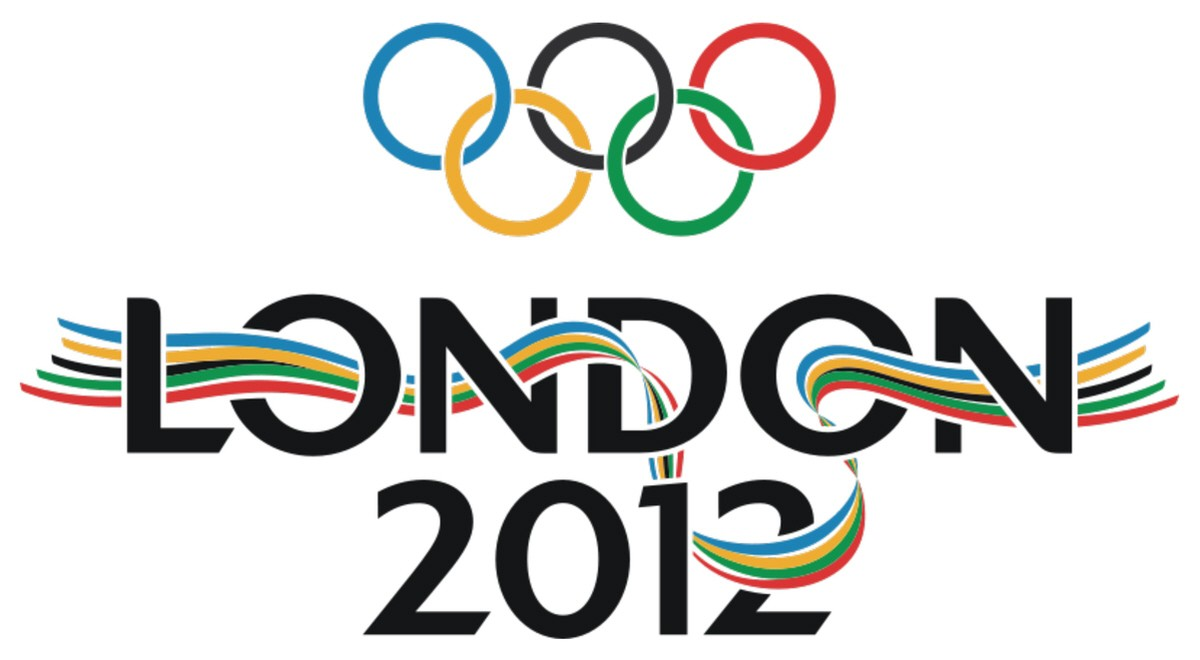
\includegraphics[scale=.6]{../graphics/london-2012-olympics-logo.jpg} \hspace{1in}

        % \setlength\fboxsep{0pt}
        % \setlength\fboxrule{0.5pt}
        % \fbox{
        % 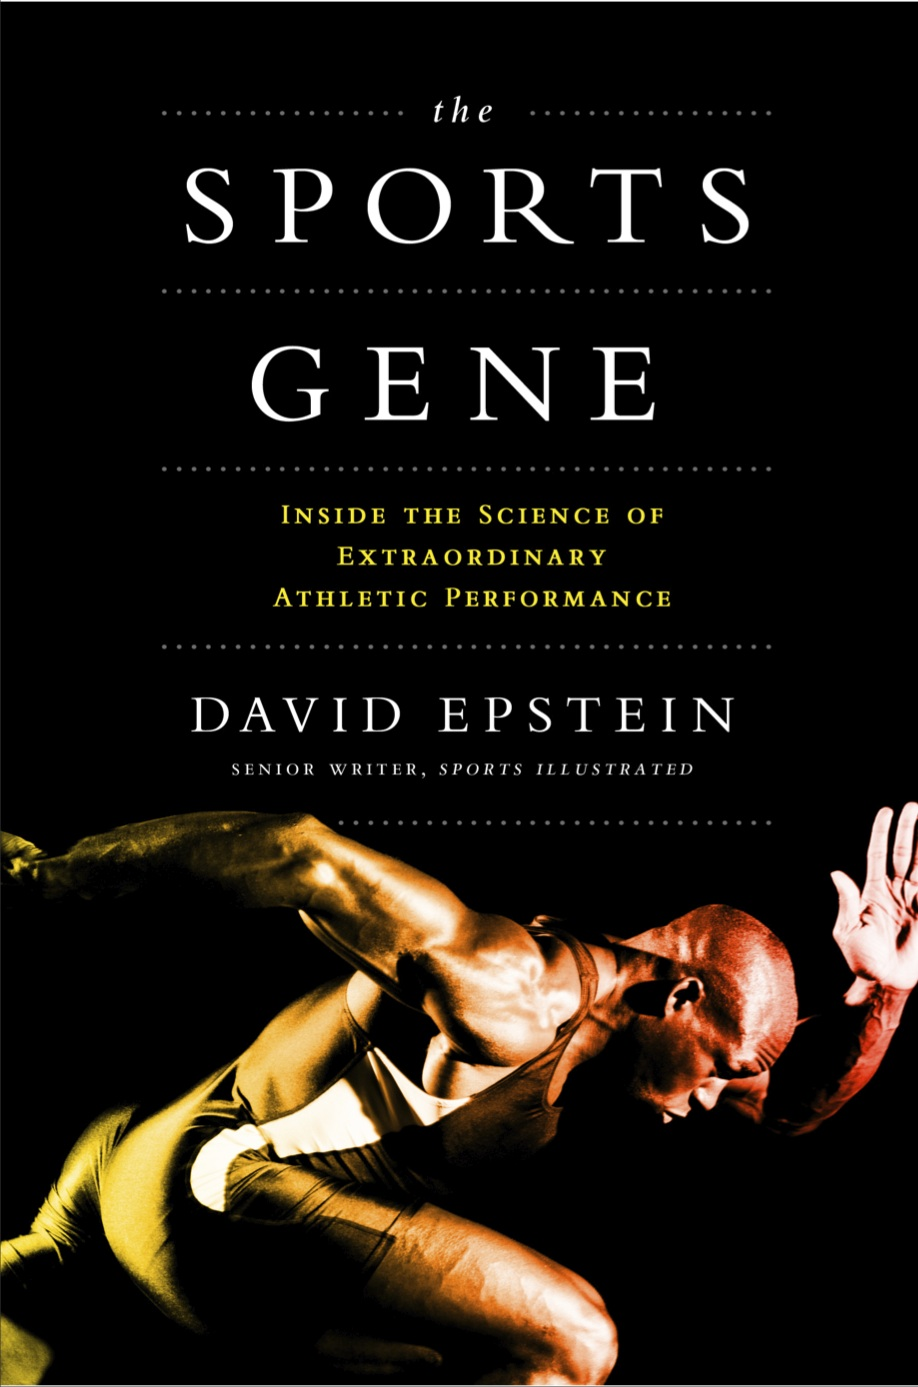
\includegraphics[scale=0.15]{../graphics/SportsGene.jpg}
        % }
\hspace{-1.5in}
} {%%% Title %%%%%%%%
% \centering
\textsf{
	\bf{Classifying Olympic Athletes By Sport and Event}}
} { %%% Authors %%%%%%%
~\\
  \hspace{-1in}
	\vspace{1em} \textsf{Matt Dickenson}\\
  %%%
  \vspace{-0.1in}
  \hspace{-1in}
	{\smaller \textsf{mcd31@duke.edu}}
} {%%% Logo %%%%%%%%%%
  % \centering 
\includegraphics[scale=.8]{dukelogo_vert_black.eps} \hspace{1in}
  \centering
  \setlength\fboxsep{0pt}
        \setlength\fboxrule{0.5pt}
        \fbox{
          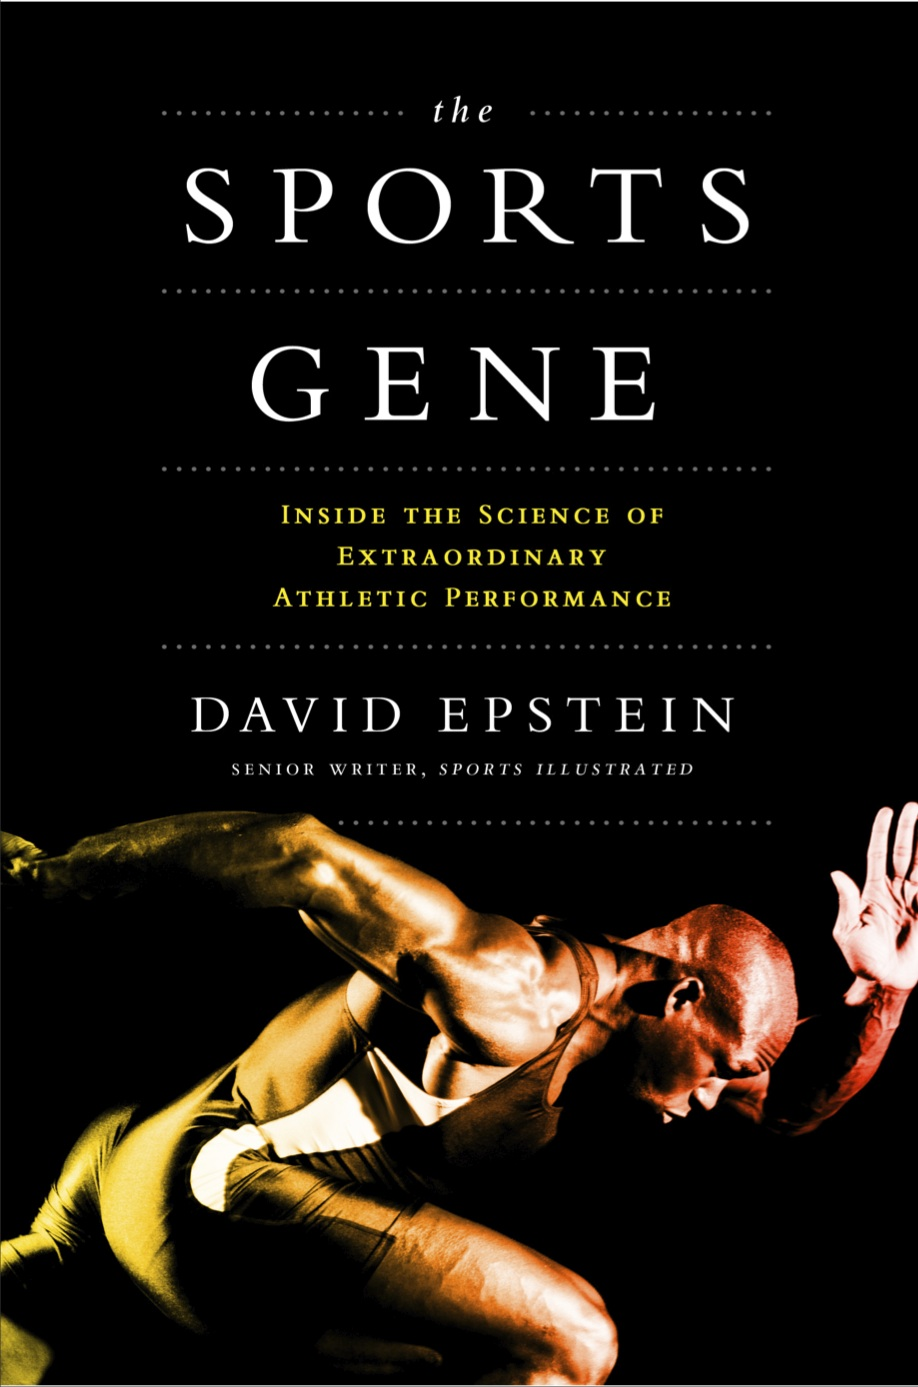
\includegraphics[scale=0.15]{../graphics/SportsGene.jpg}
        }
  % \centering 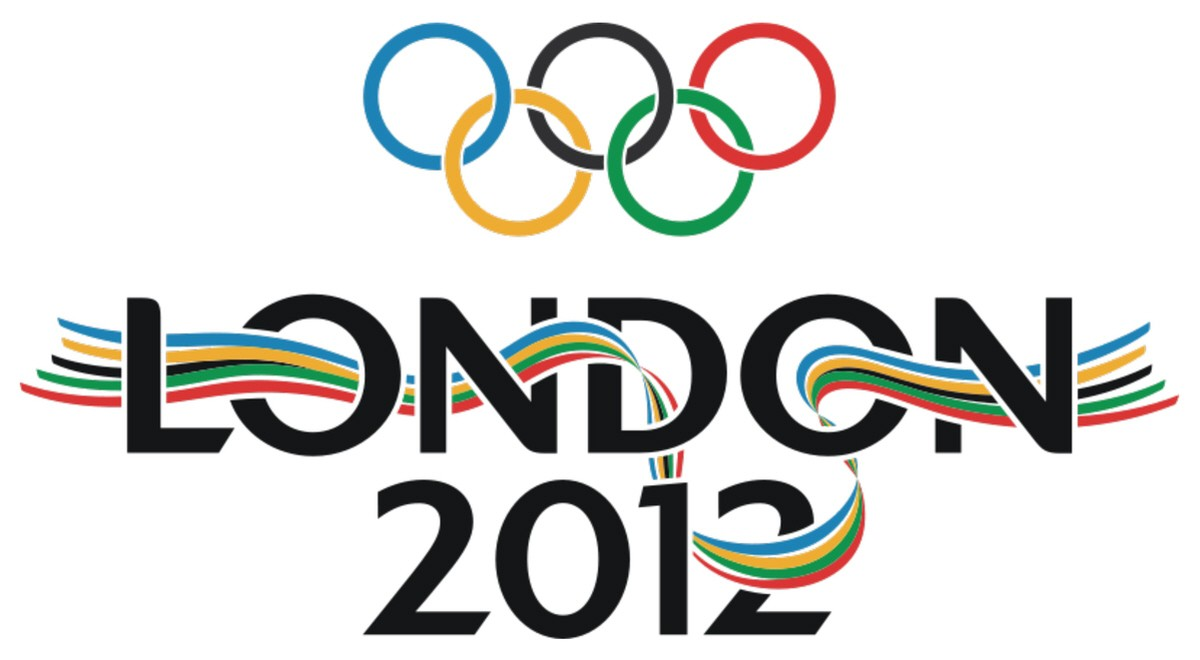
\includegraphics[scale=.6]{../graphics/london-2012-olympics-logo.jpg} 
  \hspace{1.6in}
}


%%%%%%%%%%%%%%%%%%%%%%%%%%%%%%%%%%%%%%%%%%%%%%%%%%%%%%%%%%%%%%%%%%%%%%%%%%%%%%
%%% Now define the boxes that make up the poster
%%%---------------------------------------------------------------------------
%%% Each box has a name and can be placed absolutely or relatively.
%%% The only inconvenience is that you can only specify a relative position 
%%% towards an already declared box. So if you have a box attached to the 
%%% bottom, one to the top and a third one which should be in between, you 
%%% have to specify the top and bottom boxes before you specify the middle 
%%% box.
%%%%%%%%%%%%%%%%%%%%%%%%%%%%%%%%%%%%%%%%%%%%%%%%%%%%%%%%%%%%%%%%%%%%%%%%%%%%%%
    %
    % A coloured circle useful as a bullet with an adjustably strong filling
    \newcommand{\colouredcircle}{%
      \tikz{\useasboundingbox (-0.2em,-0.32em) rectangle(0.2em,0.32em); \draw[draw=black,fill=lightblue,line width=0.03em] (0,0) circle(0.18em);}}

%%%%%%
  \headerbox{\bf Motivation}{name=question,column=0,row=0}{
%%%%%

To what extent do biological traits determine sporting success? At the highest level of amateur sports--the Olympic games--we see differences in the physical characteristics of participants across sports. Can these differences be exploited to classify individuals by sport or event given their physical attributes? 

This project was inspired by a claim made by David Epstein, author of \textit{The Sports Gene}. This claim is expressed in an interview with Russ Roberts:
\begin{quote}
\footnotesize
\textbf{Roberts}: [You argue that] if you simply had the height and weight of an Olympic roster, you could do a pretty good job of guessing what their events are. Is that correct? \\
\textbf{Epstein}: That's definitely correct. I don't think you would get every person accurately, but... \textit{I think you would get the vast majority of them correctly.} And frankly, you could definitely do it easily if you had them charted on a height-and-weight graph, and I think you could do it for most positions in something like football as well.
\end{quote}

 }

%%%%%%
  \headerbox{\bf Data}{name=data,below=question}{
%%%%%
  Data was obtained for 10,383 participants in the 2012 London Olympics from \textit{The Guardian}. The processed data consists of 8,856 complete cases. Of these, 6,956 participants were split into training ($n$=3,520) and test ($n$=3,436) sets for classification by sports ($k=27$). The remaining 1,900 Athletics participants were split into training ($n$=907) and test ($n$=993) sets for classification by event ($k=48)$. Participants' height, weight, age, and sex were used as features. Some sports and events exhibit relatively well-clustered features, whereas others are less defined.

  \begin{center}
  \begin{minipage}{0.45\textwidth}
    \begin{center}
      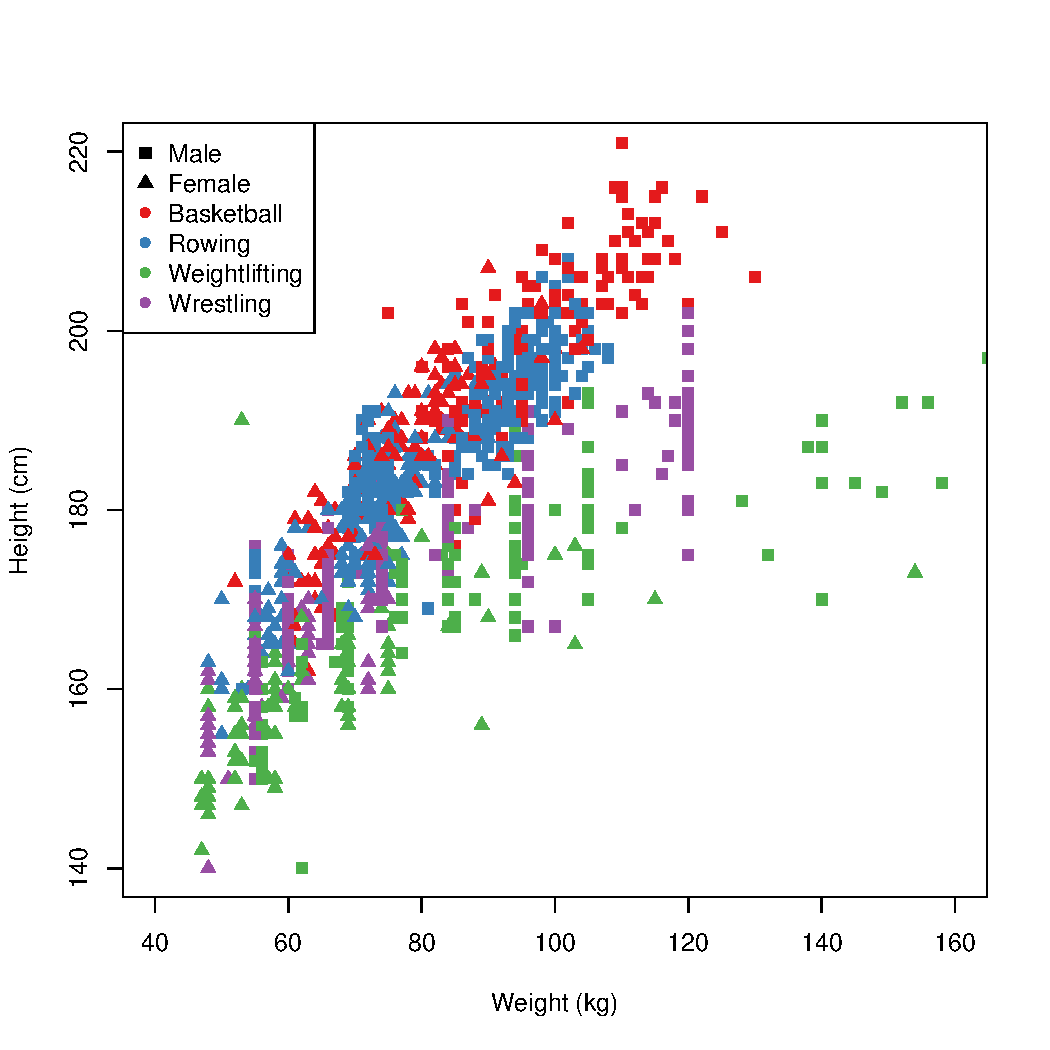
\includegraphics[scale=0.20]{../graphics/basketball.pdf}
    \end{center}
  \end{minipage}
  \hspace{0.05\textwidth}
  \begin{minipage}{0.45\textwidth}
    \begin{center}
      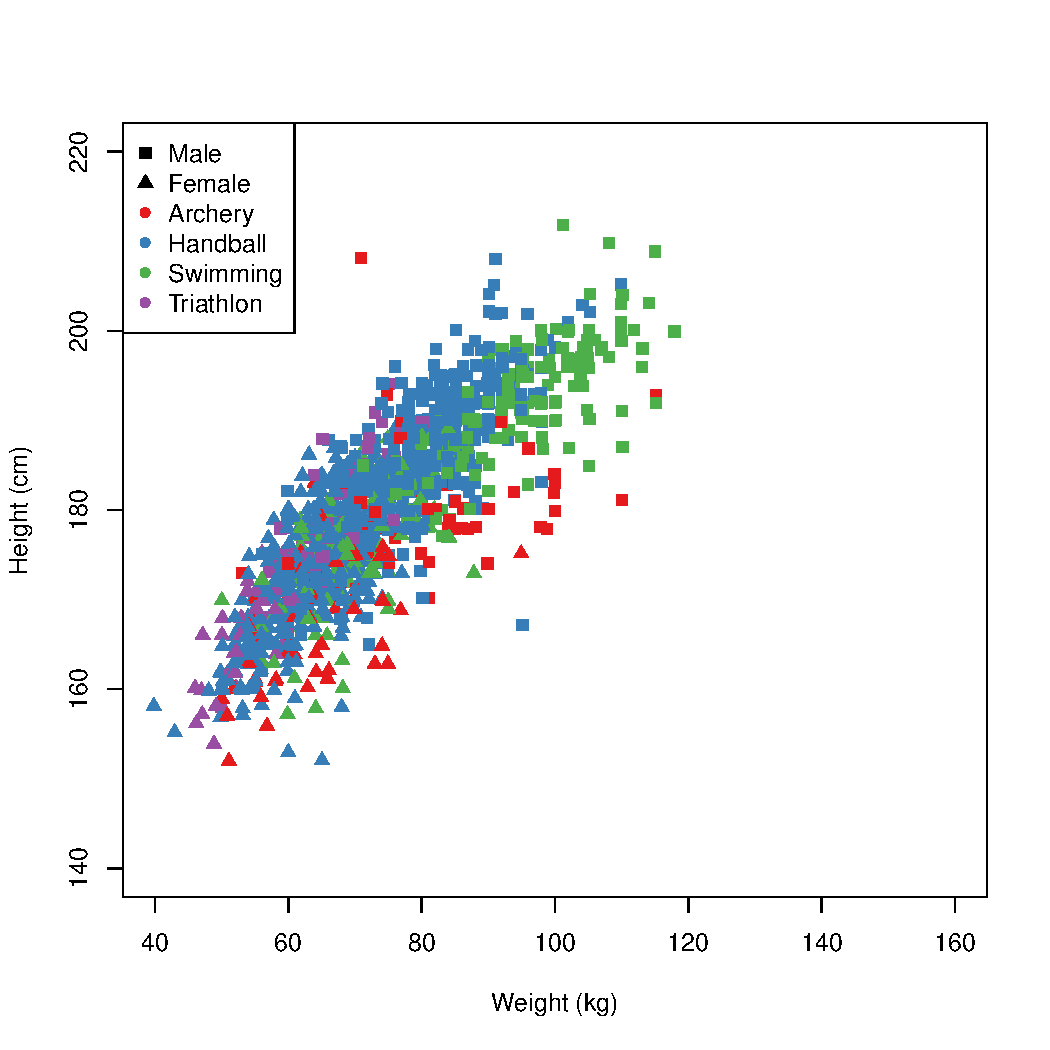
\includegraphics[scale=0.20]{../graphics/swimming.pdf}
    \end{center}
  \end{minipage}

  \begin{minipage}{0.45\textwidth}
    \begin{center}
      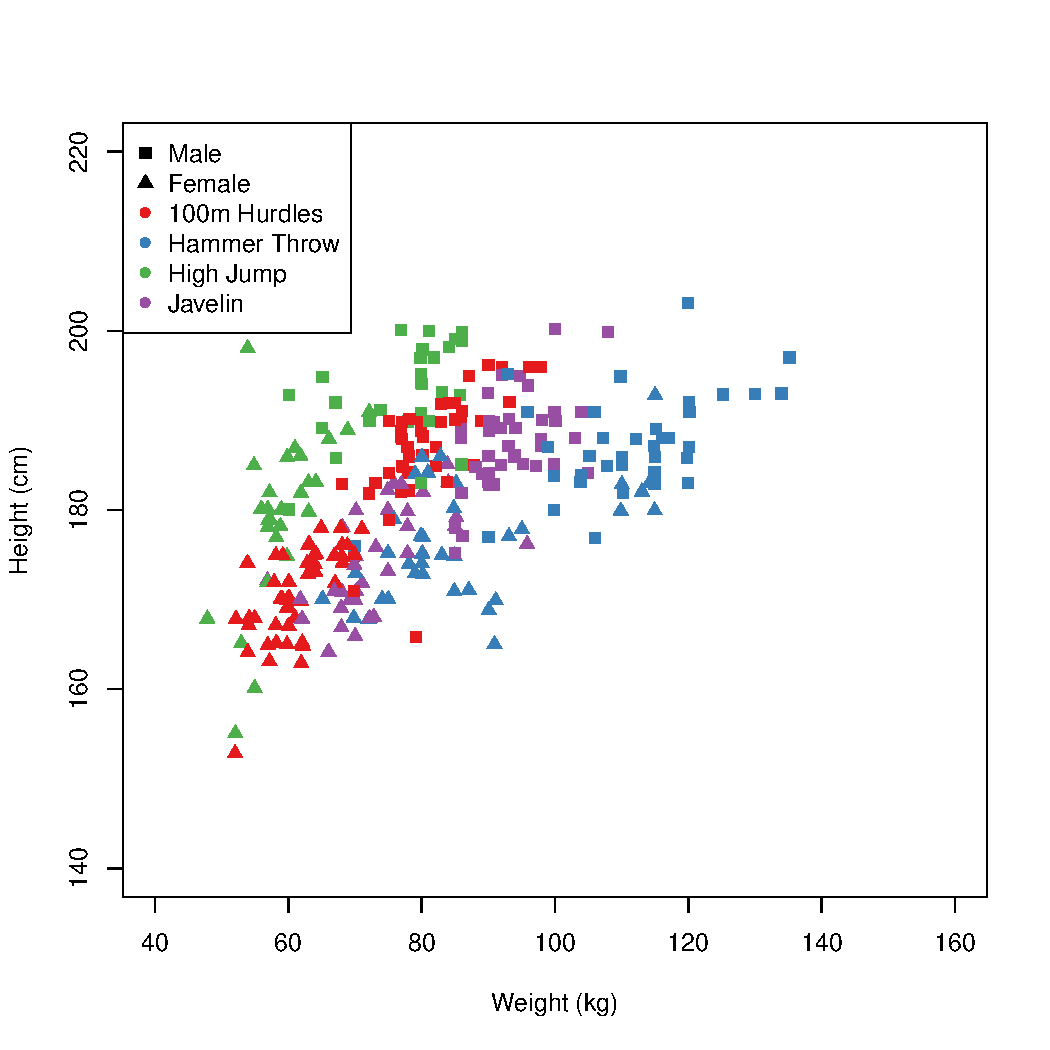
\includegraphics[scale=0.20]{../graphics/javelin.pdf}
    \end{center}
  \end{minipage}
  \hspace{0.05\textwidth}
  \begin{minipage}{0.45\textwidth}
    \begin{center}
      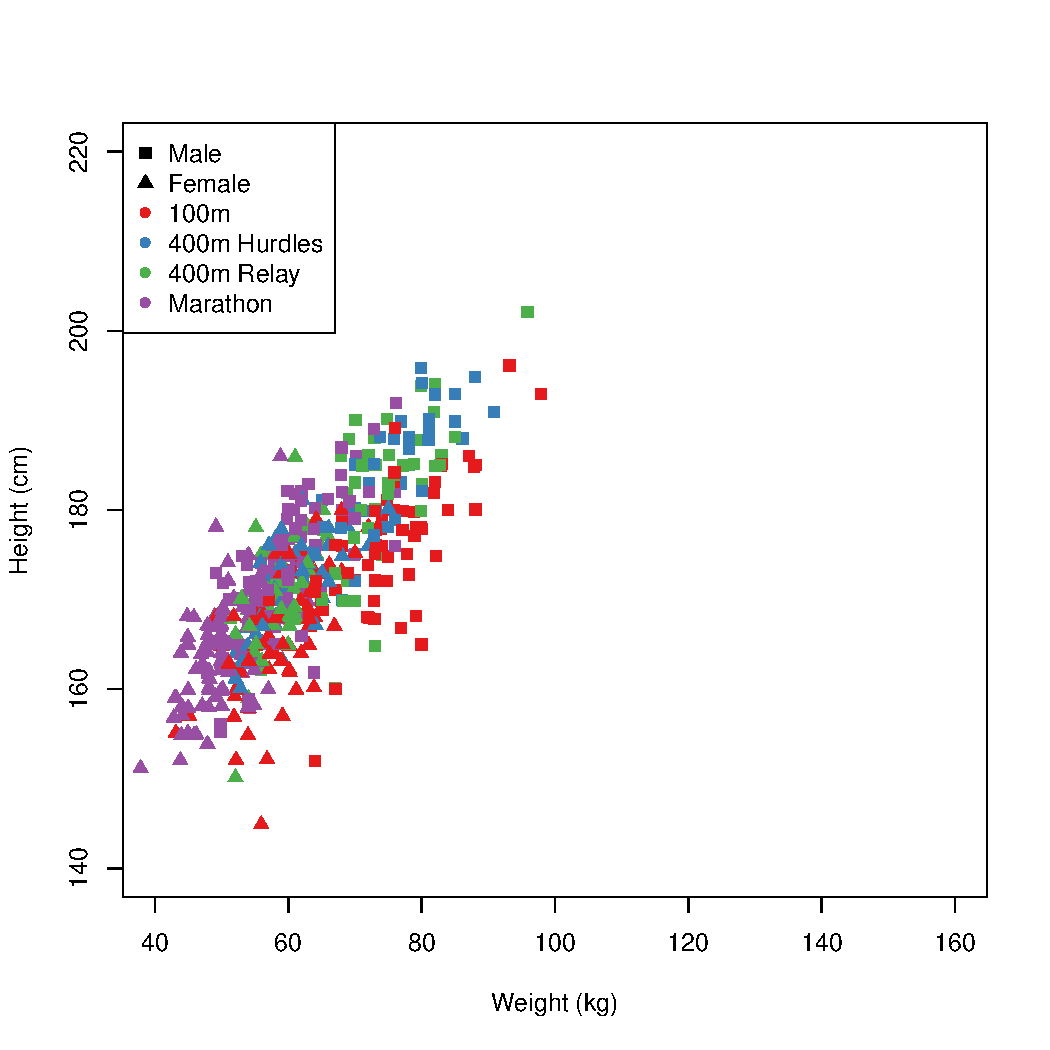
\includegraphics[scale=0.20]{../graphics/marathon.pdf}
    \end{center}
  \end{minipage}
  \end{center}
 }

%%%%%%
  \headerbox{\bf Methodology}{name=methods,below=data,above=bottom}{
%%%%%
  Several machine learning methods were applied to this classification problem. Conditional inference trees were formed by recursive binary partitioning. Evolutionary trees were constructed to be globally optimal by minimizing the misclassification rate. Breiman's Random Forest algorithm was used with 500 trees. Single-hidden-layer neural networks were constructed with 30 units in the hidden layer for sport classification and 50 for event classification.
  % Hierarchical clustering using Gaussian marginal likelihoods was performed using the \texttt{mclust} package.

  % \begin{center}
  %   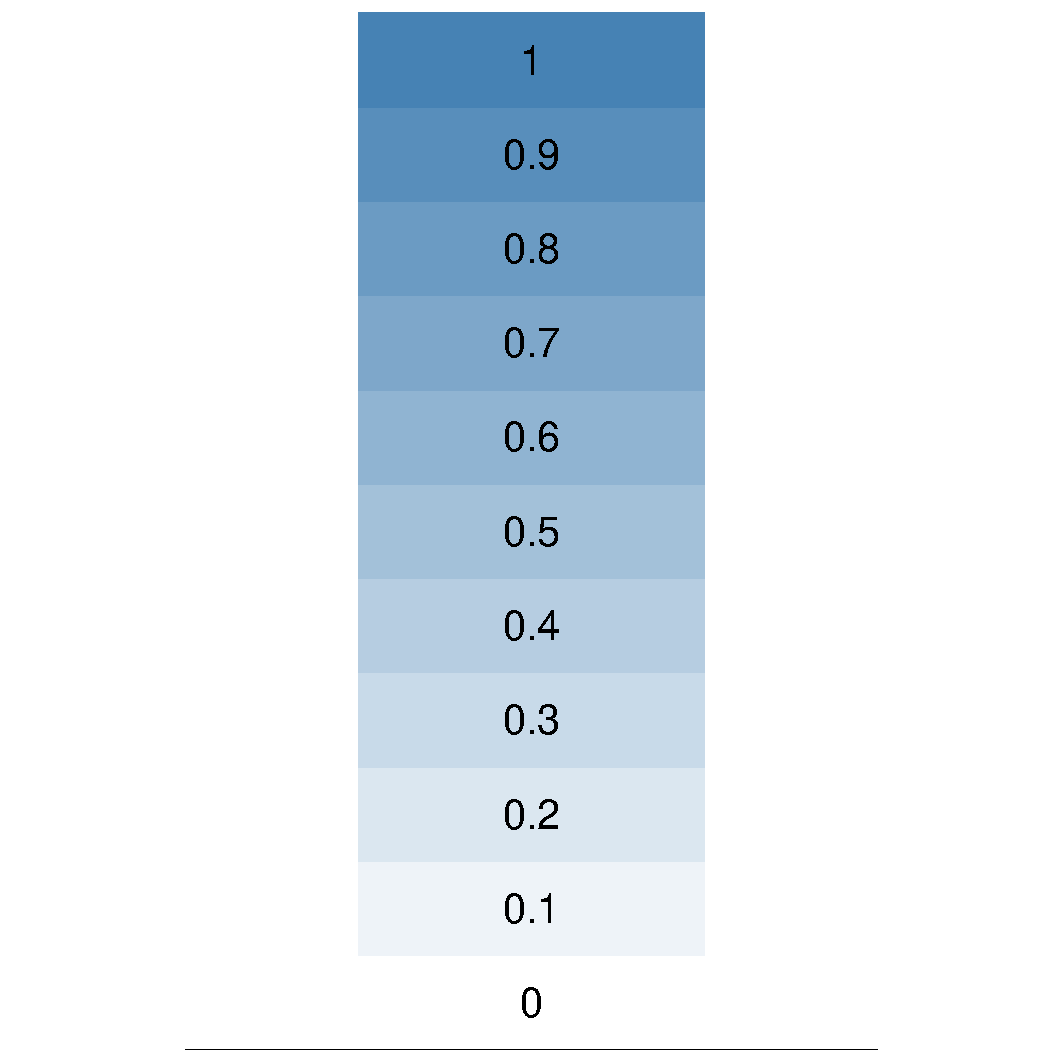
\includegraphics[scale=0.2]{../graphics/scale.pdf}
  % \end{center}

  \vspace{0.1in}

  \begin{minipage}{0.4\textwidth}
        \begin{center}
    % \hspace{-1.5in}
      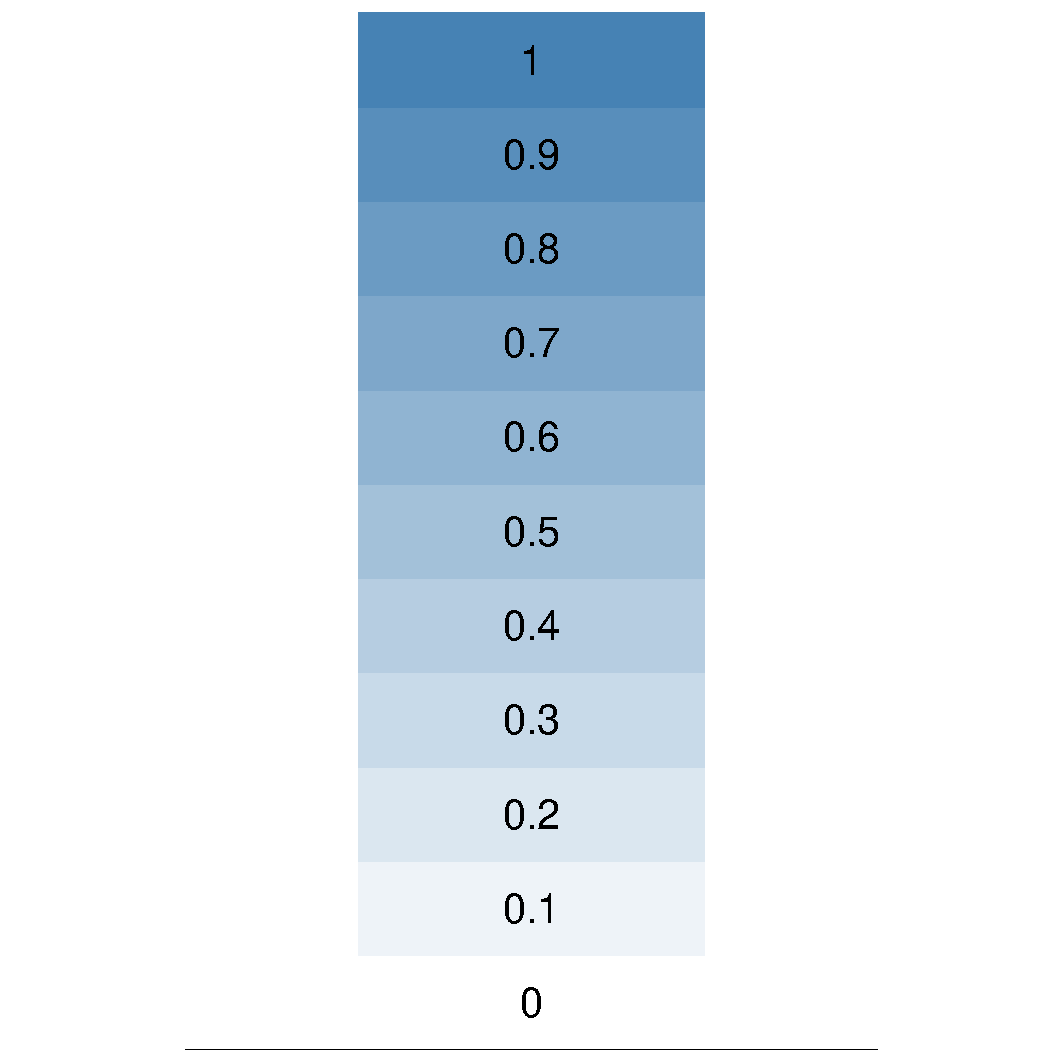
\includegraphics[scale=0.2]{../graphics/scale.pdf}
    \hspace{-0.5in}
    \end{center}
  \end{minipage}
  \hspace{0.05\textwidth}
  \begin{minipage}{0.45\textwidth}
    The columns at right present the results visually, with row-normalized observed frequencies. The figure at left serves as a legend for all heatmaps.
  \end{minipage}
  % todo: fix the scale
 }


%%%%%%
  \headerbox{\bf Classification by Sport}{name=estimations,column=1,row=0}{
%%%%%

  \begin{center}
  % %%%%%%%%%%%%%%%%%%%%%%%%%%%%%%%%%%%%%%%%%%%%%%%%%%%%%%%%
  % Hierarchical Clustering \\
  % \begin{minipage}{0.45\textwidth}
  %   \begin{center}
  %     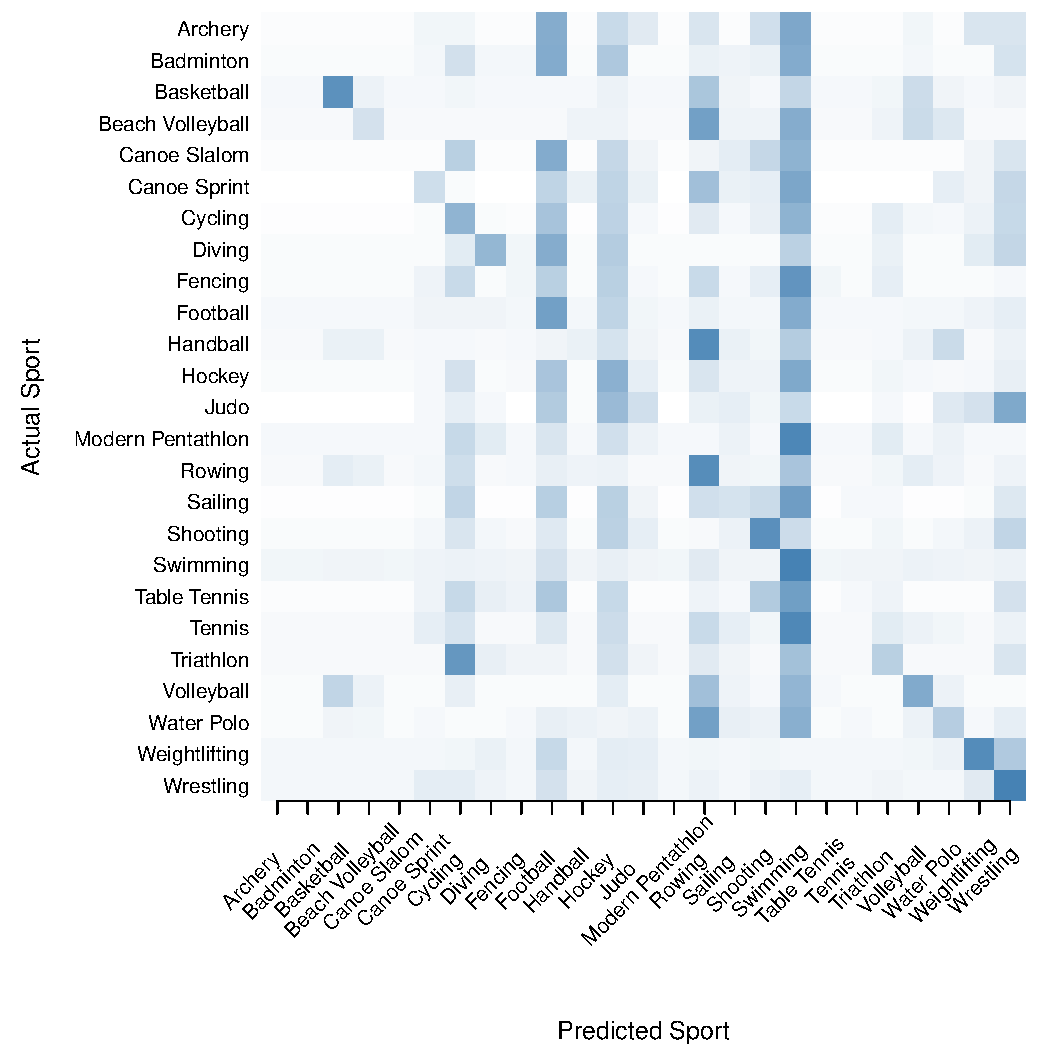
\includegraphics[scale=0.27]{../graphics/sportMclust-trn.pdf}
  %   \end{center}
  % \end{minipage}
  % \hspace{0.05\textwidth}
  % \begin{minipage}{0.45\textwidth}
  %   \begin{center}
  %     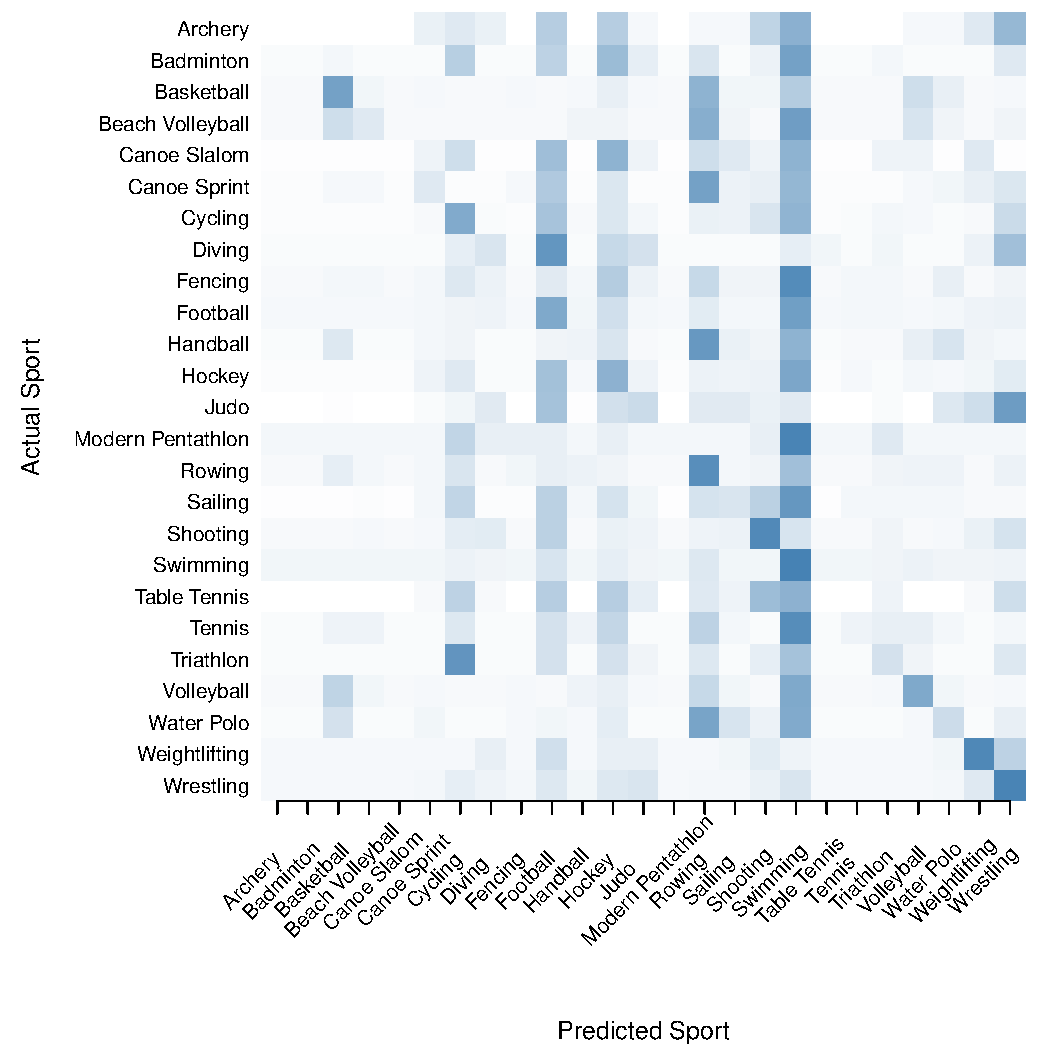
\includegraphics[scale=0.27]{../graphics/sportMclust-tst.pdf}
  %   \end{center}
  % \end{minipage}


  %%%%%%%%%%%%%%%%%%%%%%%%%%%%%%%%%%%%%%%%%%%%%%%%%%%%%%%%%
    Conditional Inference Tree \\

  \begin{minipage}{0.45\textwidth}
    \begin{center}
      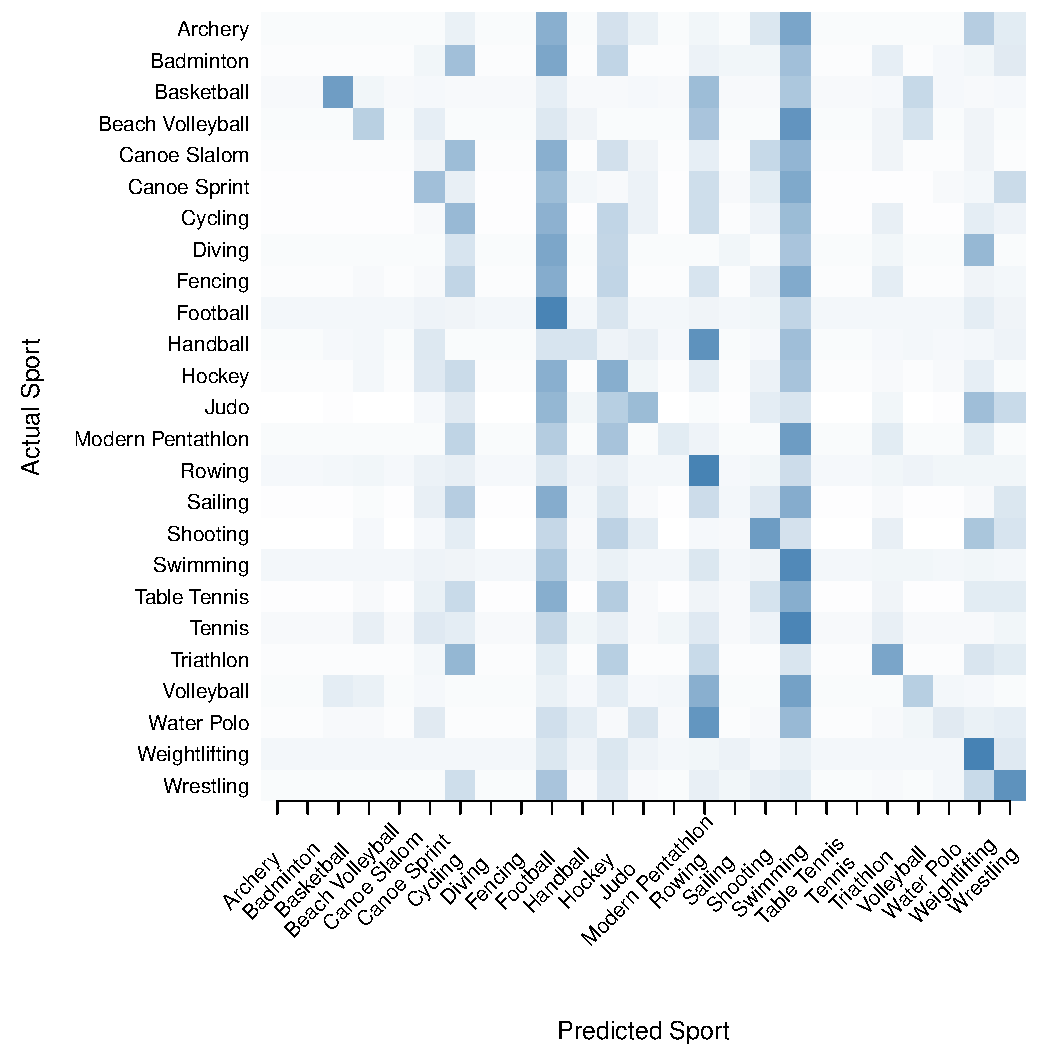
\includegraphics[scale=0.27]{../graphics/sportCIT-trn.pdf}
    \end{center}
  \end{minipage}
  \hspace{0.05\textwidth}
  \begin{minipage}{0.45\textwidth}
    \begin{center}
      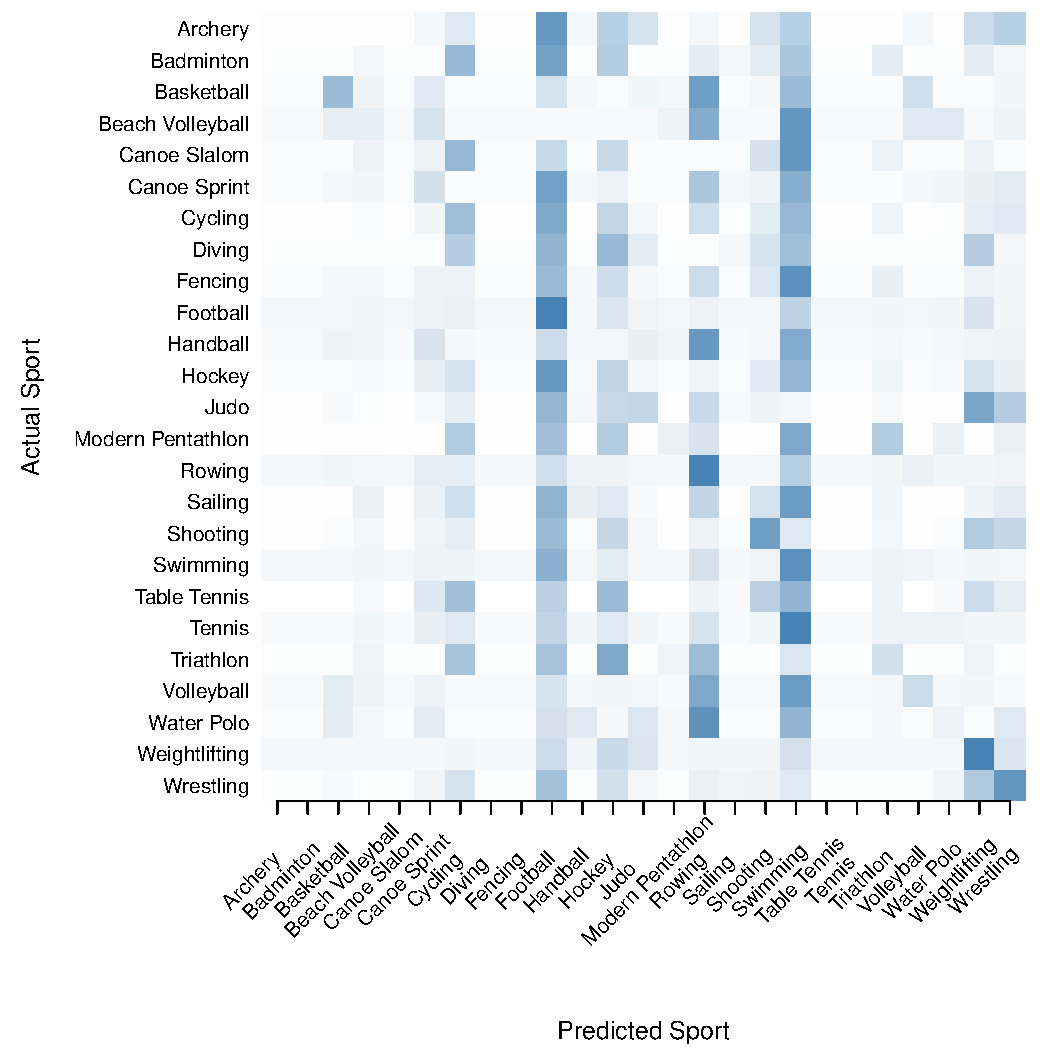
\includegraphics[scale=0.27]{../graphics/sportCIT-tst.pdf}
    \end{center}
  \end{minipage}



  %%%%%%%%%%%%%%%%%%%%%%%%%%%%%%%%%%%%%%%%%%%%%%%%%%%%%%%%%
    Evolutionary Tree \\

  \begin{minipage}{0.45\textwidth}
    \begin{center}
      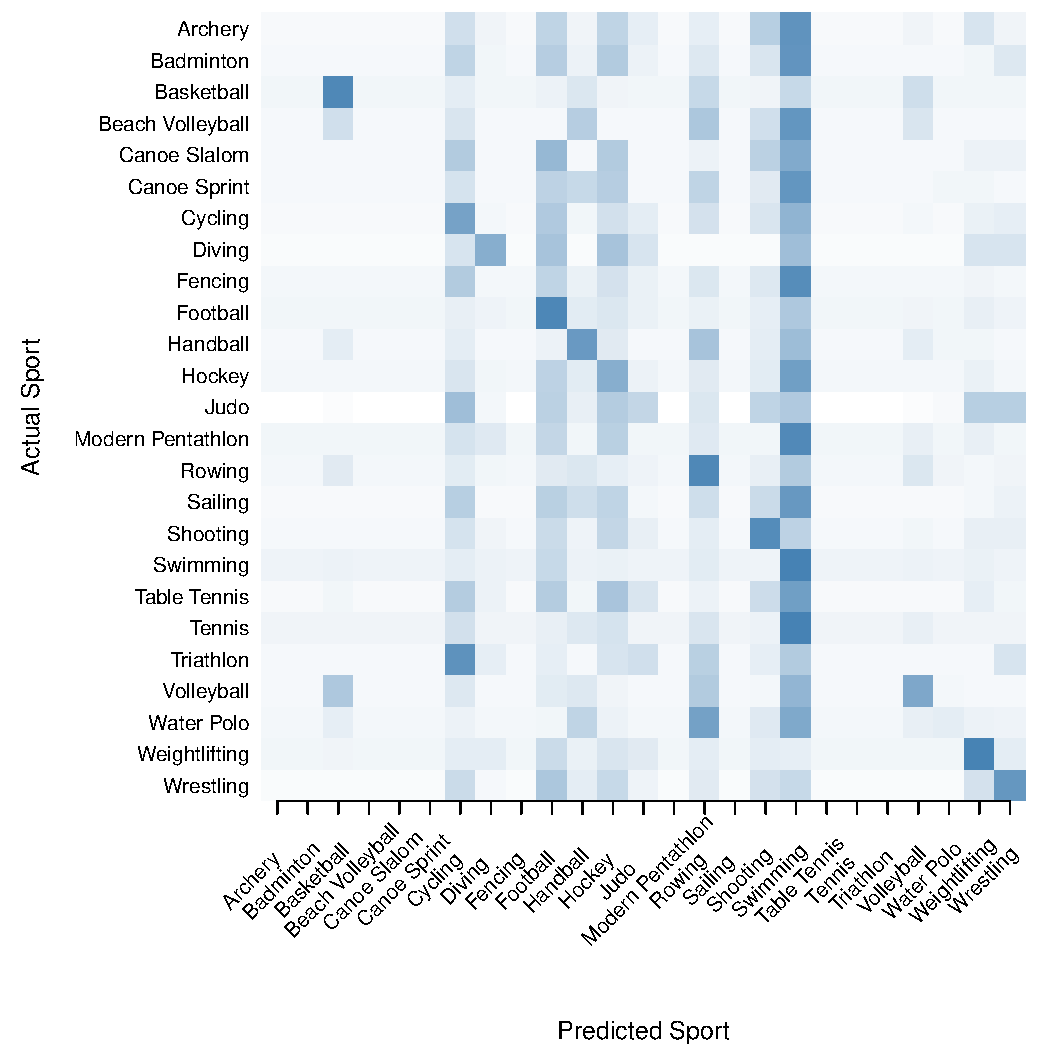
\includegraphics[scale=0.27]{../graphics/sportEV-trn.pdf}
    \end{center}
  \end{minipage}
  \hspace{0.05\textwidth}
  \begin{minipage}{0.45\textwidth}
    \begin{center}
      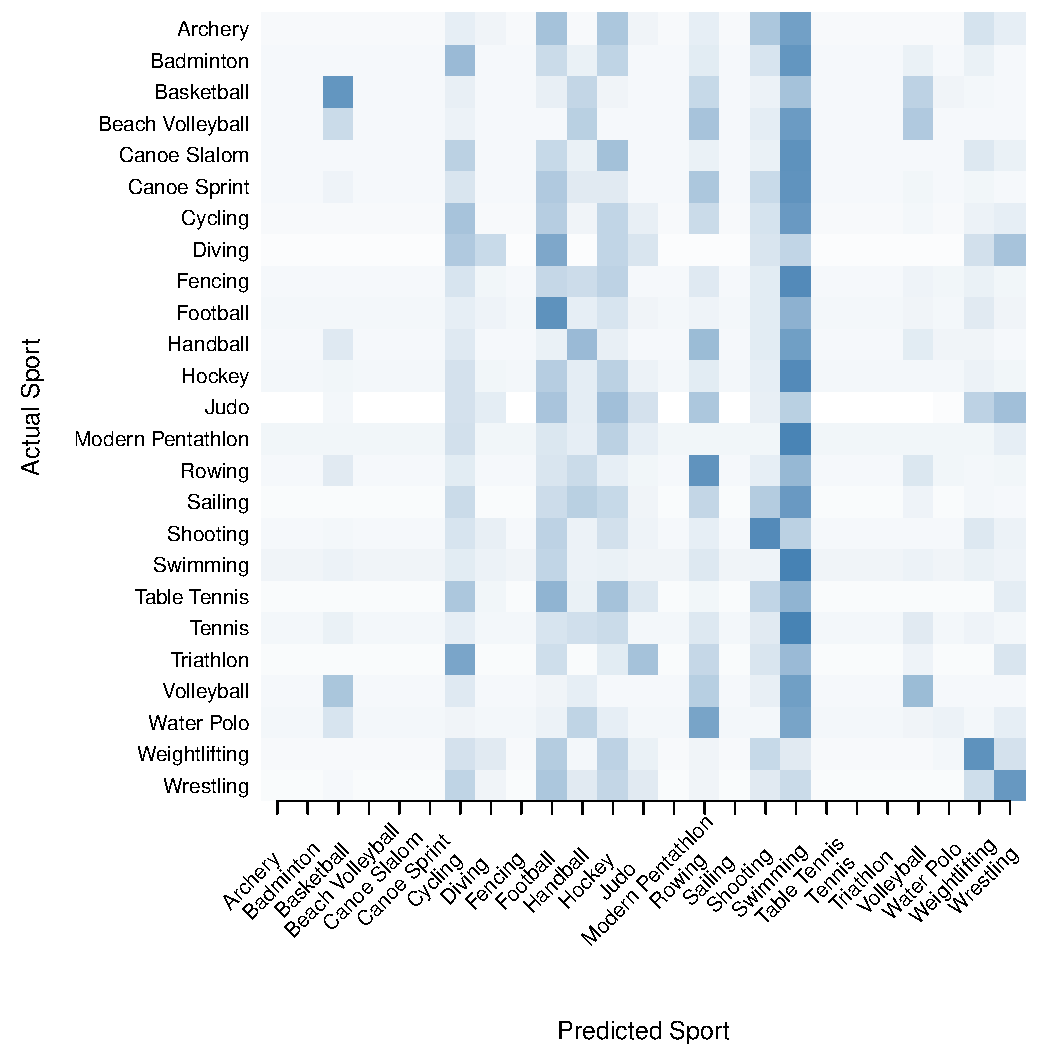
\includegraphics[scale=0.27]{../graphics/sportEV-tst.pdf}
    \end{center}
  \end{minipage}



  %%%%%%%%%%%%%%%%%%%%%%%%%%%%%%%%%%%%%%%%%%%%%%%%%%%%%%%%%
    Random Forest \\
  \begin{minipage}{0.45\textwidth}
    \begin{center}
      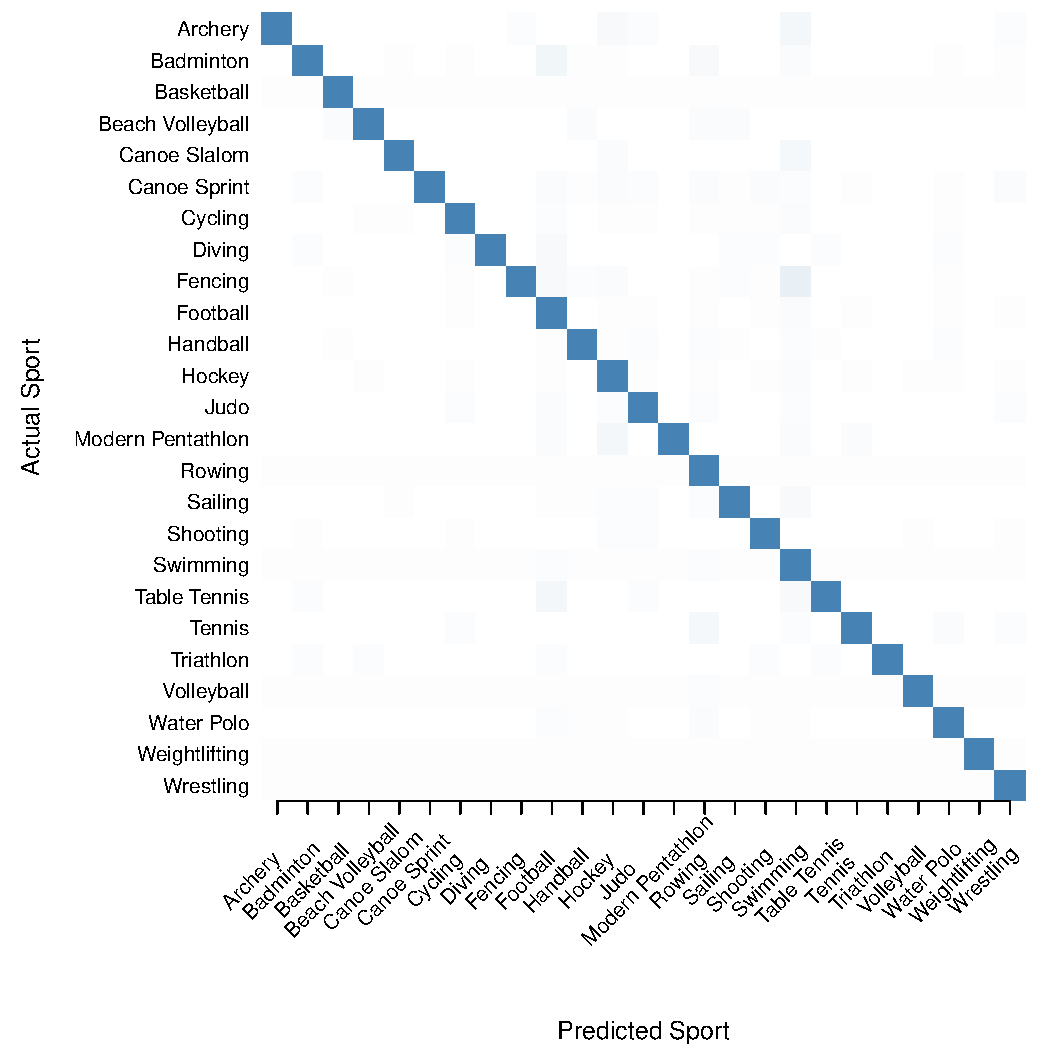
\includegraphics[scale=0.27]{../graphics/sportRF-trn.pdf}
    \end{center}
  \end{minipage}
  \hspace{0.05\textwidth}
  \begin{minipage}{0.45\textwidth}
    \begin{center}
      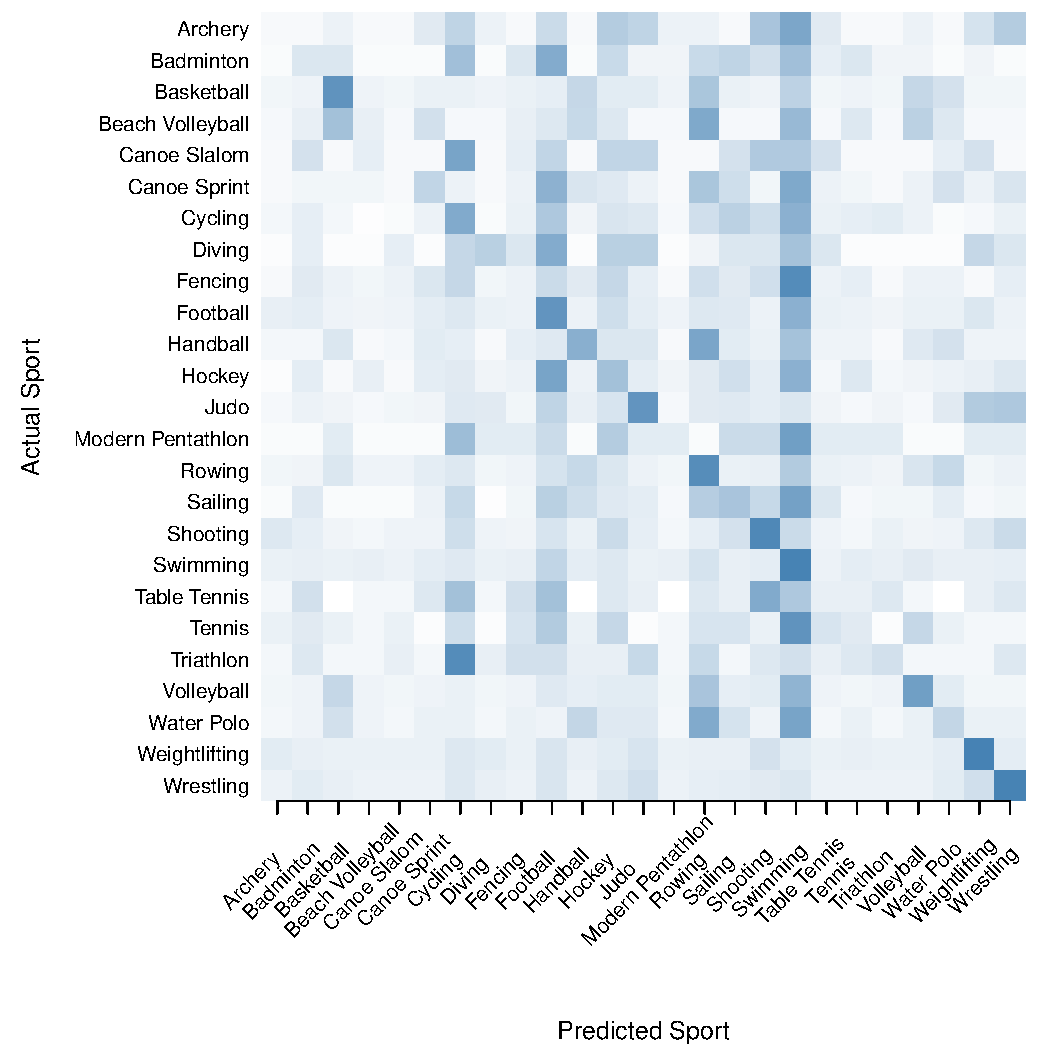
\includegraphics[scale=0.27]{../graphics/sportRF-tst.pdf}
    \end{center}
  \end{minipage}



  %%%%%%%%%%%%%%%%%%%%%%%%%%%%%%%%%%%%%%%%%%%%%%%%%%%%%%%%%
    Neural Network \\
  \begin{minipage}{0.45\textwidth}
    \begin{center}
      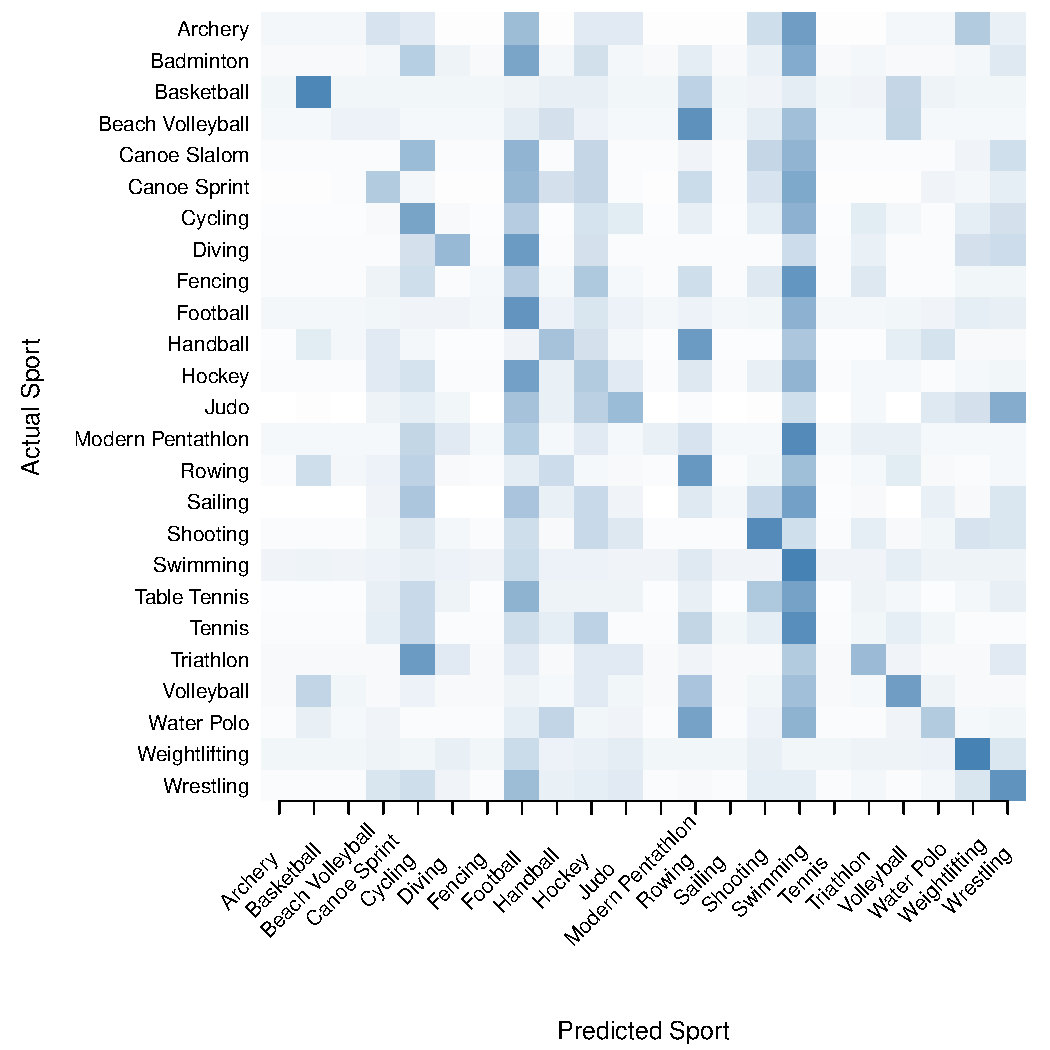
\includegraphics[scale=0.27]{../graphics/sportANN-trn.pdf}
    \end{center}
  \end{minipage}
  \hspace{0.05\textwidth}
  \begin{minipage}{0.45\textwidth}
    \begin{center}
      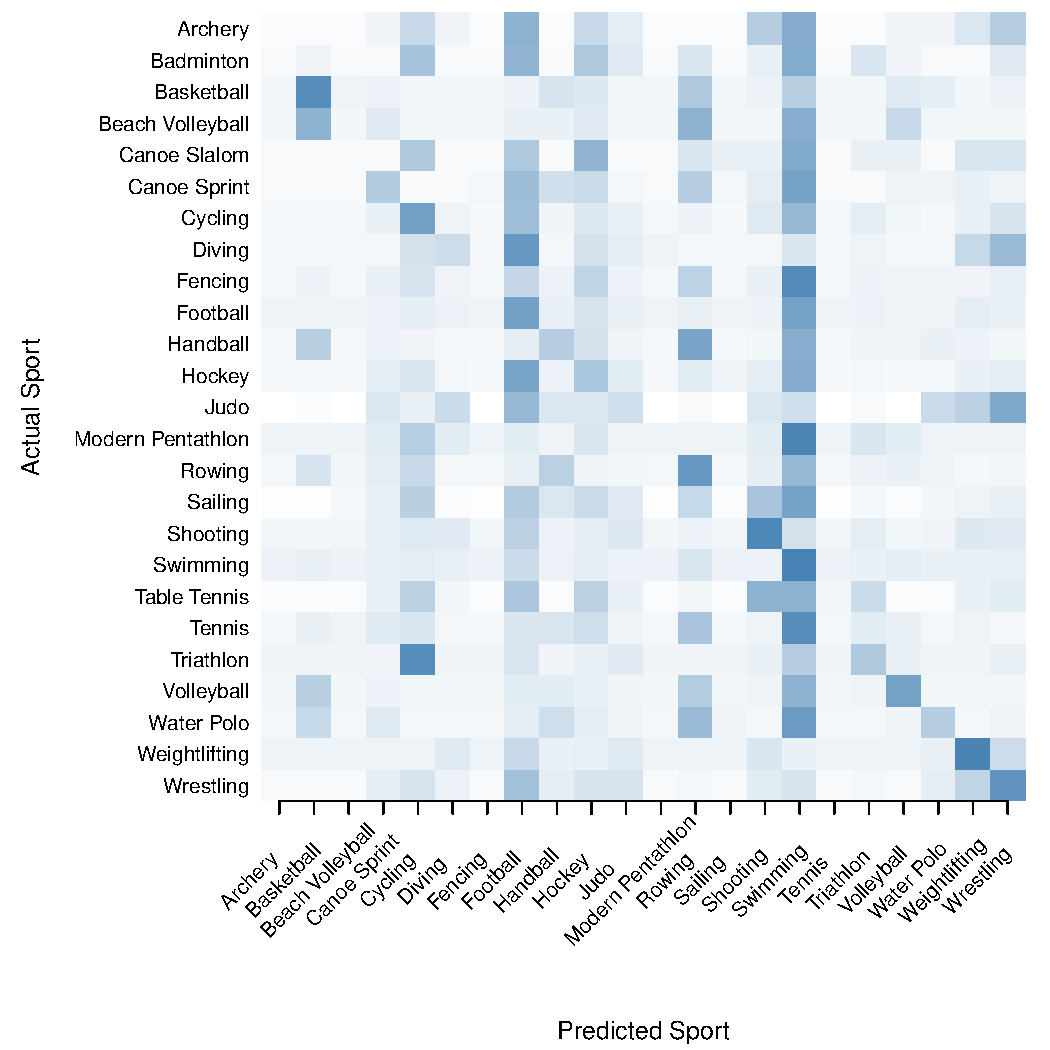
\includegraphics[scale=0.27]{../graphics/sportANN-tst.pdf}
    \end{center}
  \end{minipage}
  \end{center}



 }

 %%%%%%
  \headerbox{\bf Accuracy}{name=accuracy,below=estimations,above=bottom,column=1}{
%%%%%
 Evolutionary trees and neural networks both exhibit higher accuracy for events than sports, and maintain acceptable out-of-sample accuracy. Conditional inference trees do slightly less well for both training and test sets. Random forests tend to overfit the training data but still do well on the test set. Overall, this appears to be a difficult classification problem.

\vspace{-0.05in}
  \begin{center}
  \footnotesize
    \begin{tabular}{lcccccc}
      \multicolumn{1}{c}{} & \multicolumn{3}{c}{Sports} & \multicolumn{3}{c}{Events} \\
       \multicolumn{1}{c}{} & \multicolumn{1}{c}{Train} & \multicolumn{1}{c}{Test} & \multicolumn{1}{c}{Ratio} & \multicolumn{1}{c}{Train} & \multicolumn{1}{c}{Test} & \multicolumn{1}{c}{Ratio}\\
      \midrule
      % \footnotesize{Hierarchical Clustering}     & .272 & .271 & .998 \\
      Conditional Inference Tree  & .279 & .219 & .784 & .277 & .218 & .787 \\
      Evolutionary Tree           & .292 & .236 & .807 & .303 & .230 & .757 \\
      Random Forest               & .923 & .244 & .265 & .976 & .228 & .233 \\
      Neural Network              & .280 & .265 & .949 & .397 & .249 & .623
    \end{tabular}
  \end{center}
 }


%%%%%%
  \headerbox{\bf Classification by Event}{name=predictions,column=2,row=0}{
%%%%%
  
    %%%%%%%%%%%%%%%%%%%%%%%%%%%%%%%%%%%%%%%%%%%%%%%%%%%%%%%%%
\begin{center}
  Conditional Inference Tree \\
  \begin{minipage}{0.45\textwidth}
    \begin{center}
      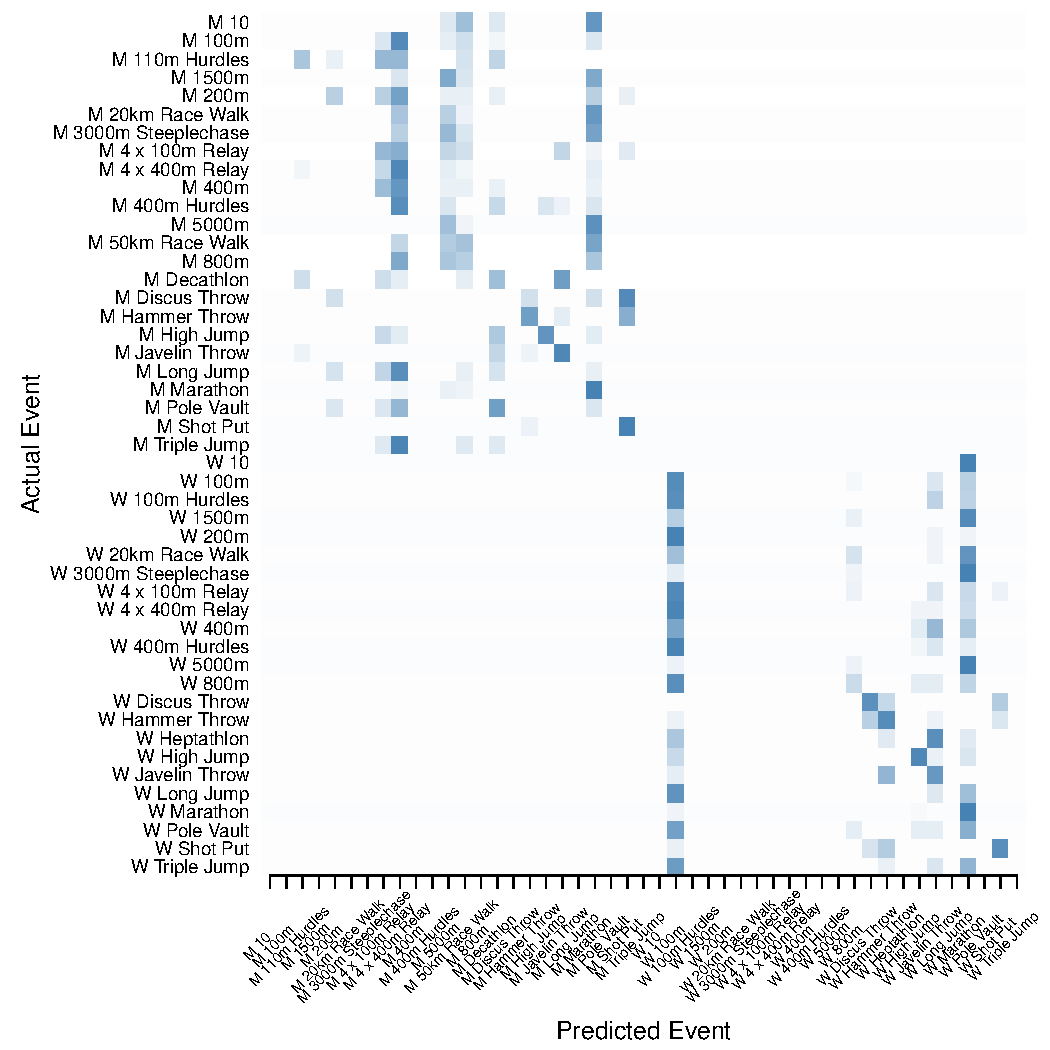
\includegraphics[scale=0.27]{../graphics/athletesCIT-trn.pdf}
    \end{center}
  \end{minipage}
  \hspace{0.05\textwidth}
  \begin{minipage}{0.45\textwidth}
    \begin{center}
      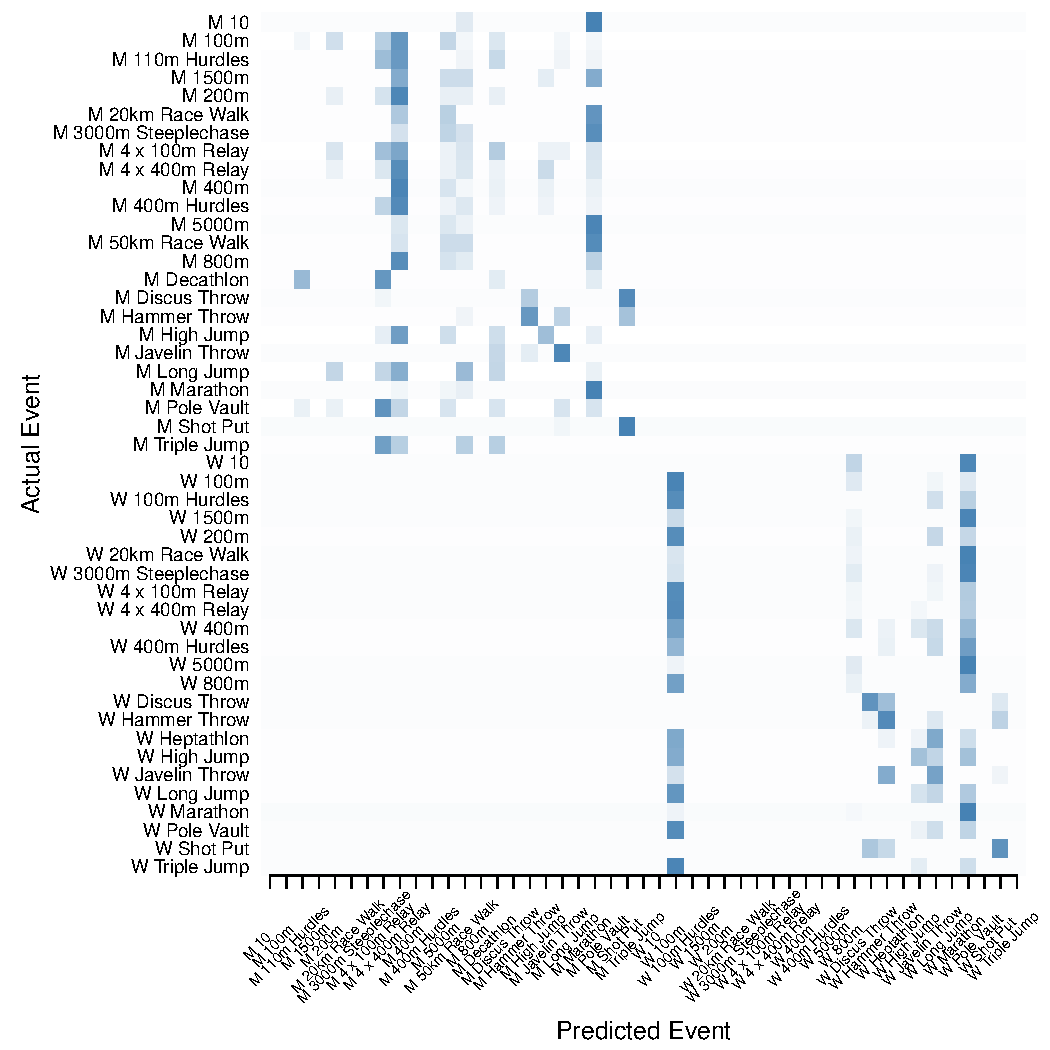
\includegraphics[scale=0.27]{../graphics/athletesCIT-tst.pdf}
    \end{center}
  \end{minipage}


  %%%%%%%%%%%%%%%%%%%%%%%%%%%%%%%%%%%%%%%%%%%%%%%%%%%%%%%%%
  Evolutionary Tree \\
  \begin{minipage}{0.45\textwidth}
    \begin{center}
      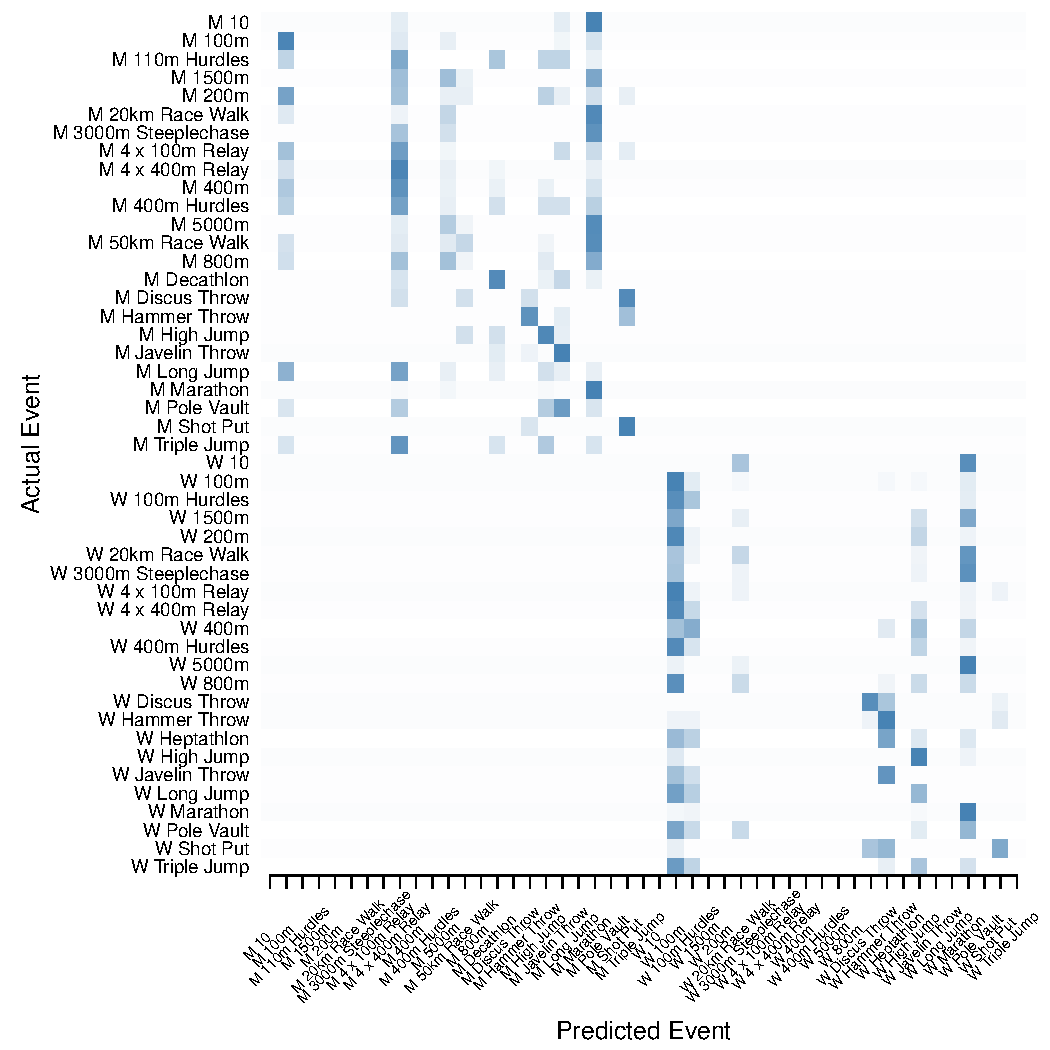
\includegraphics[scale=0.27]{../graphics/athletesEV-trn.pdf}
    \end{center}
  \end{minipage}
  \hspace{0.05\textwidth}
  \begin{minipage}{0.45\textwidth}
    \begin{center}
      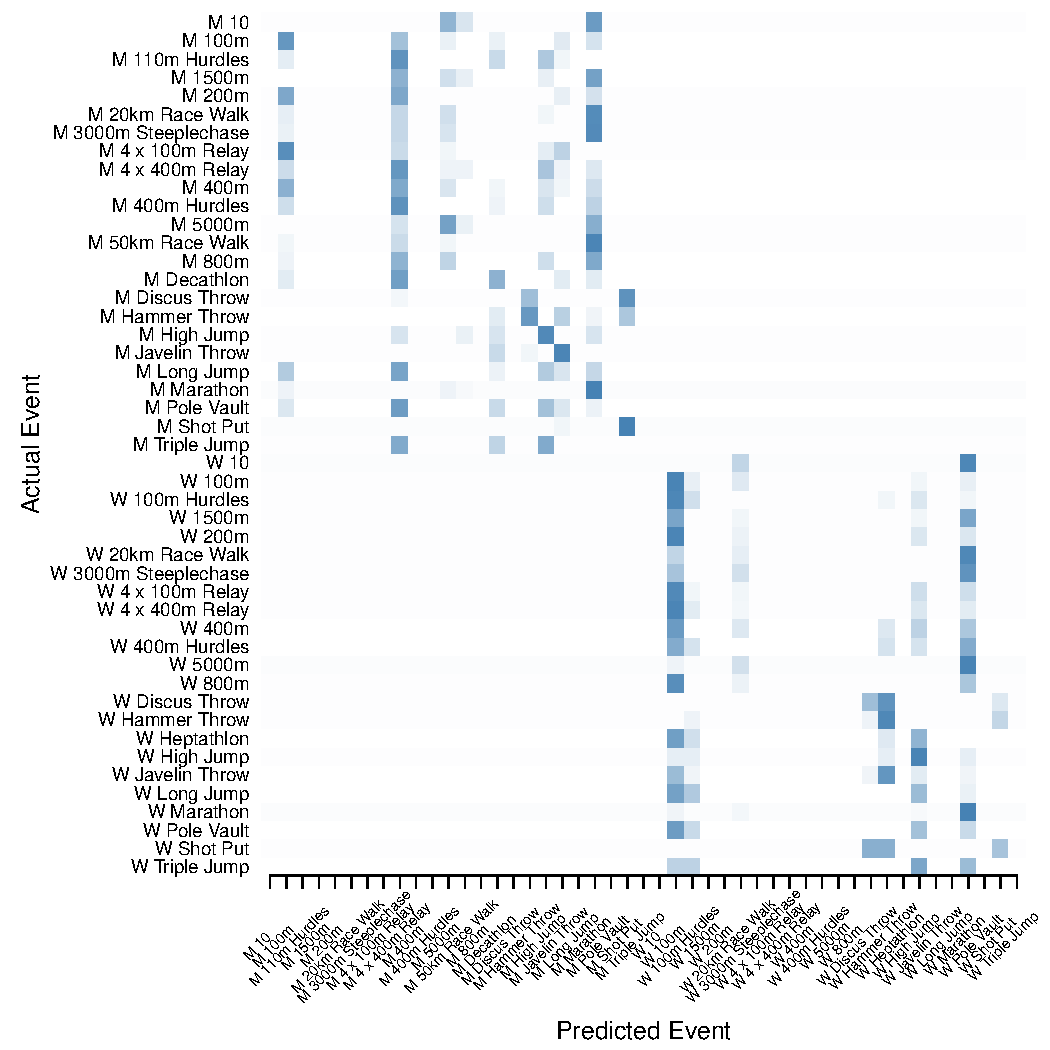
\includegraphics[scale=0.27]{../graphics/athletesEV-tst.pdf}
    \end{center}
  \end{minipage}


  %%%%%%%%%%%%%%%%%%%%%%%%%%%%%%%%%%%%%%%%%%%%%%%%%%%%%%%%%
  Random Forest \\
  \begin{minipage}{0.45\textwidth}
    \begin{center}
      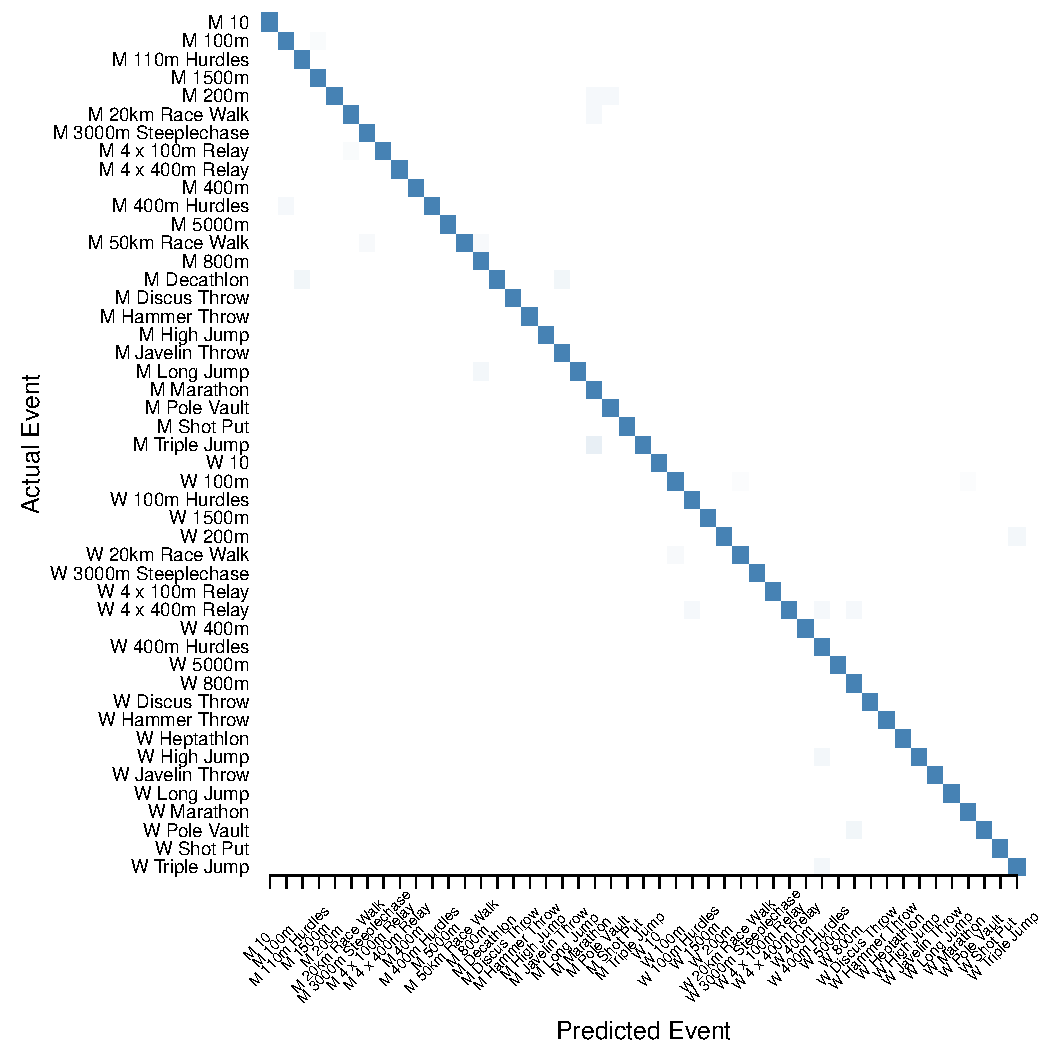
\includegraphics[scale=0.27]{../graphics/athletesRF-trn.pdf}
    \end{center}
  \end{minipage}
  \hspace{0.05\textwidth}
  \begin{minipage}{0.45\textwidth}
    \begin{center}
      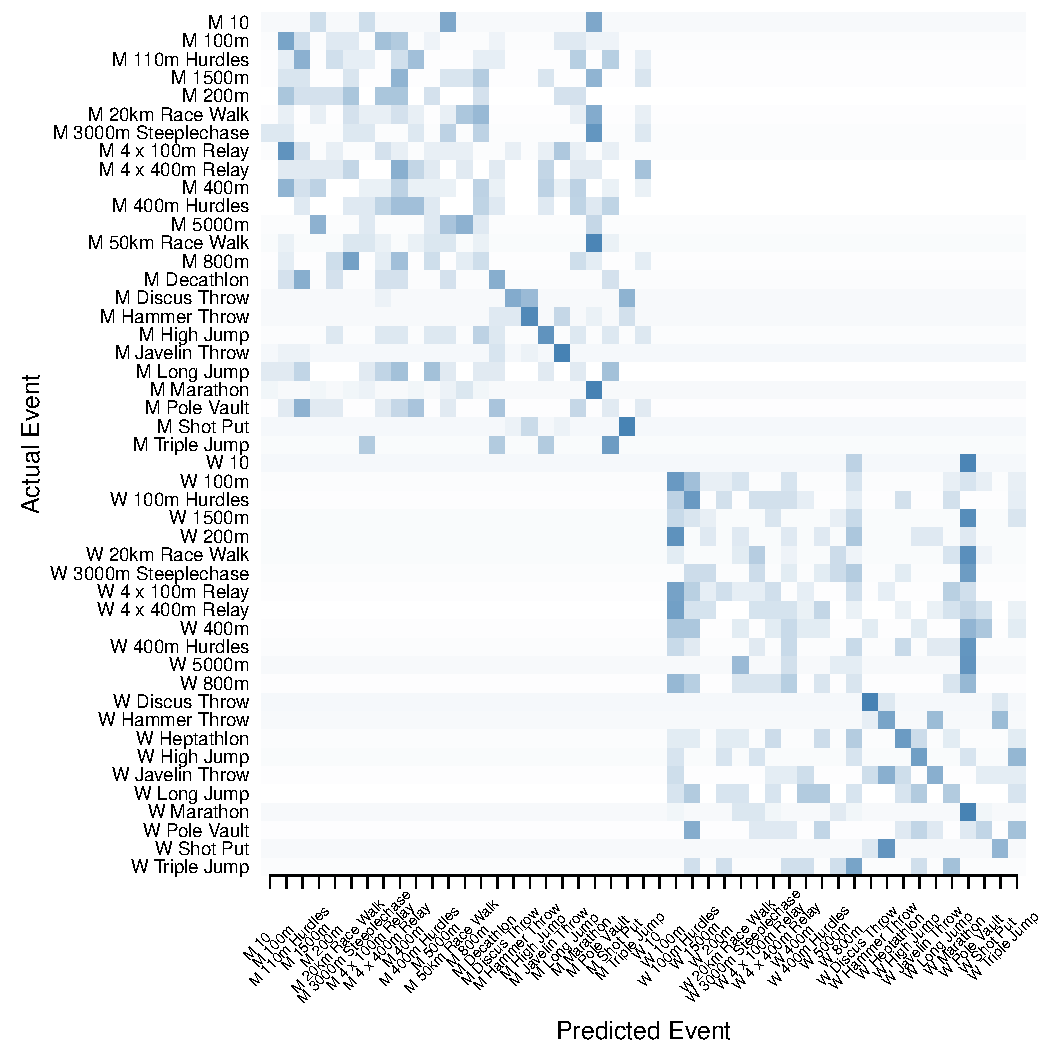
\includegraphics[scale=0.27]{../graphics/athletesRF-tst.pdf}
    \end{center}
  \end{minipage}


  %%%%%%%%%%%%%%%%%%%%%%%%%%%%%%%%%%%%%%%%%%%%%%%%%%%%%%%%%
  Neural Network \\
  \begin{minipage}{0.45\textwidth}
    \begin{center}
      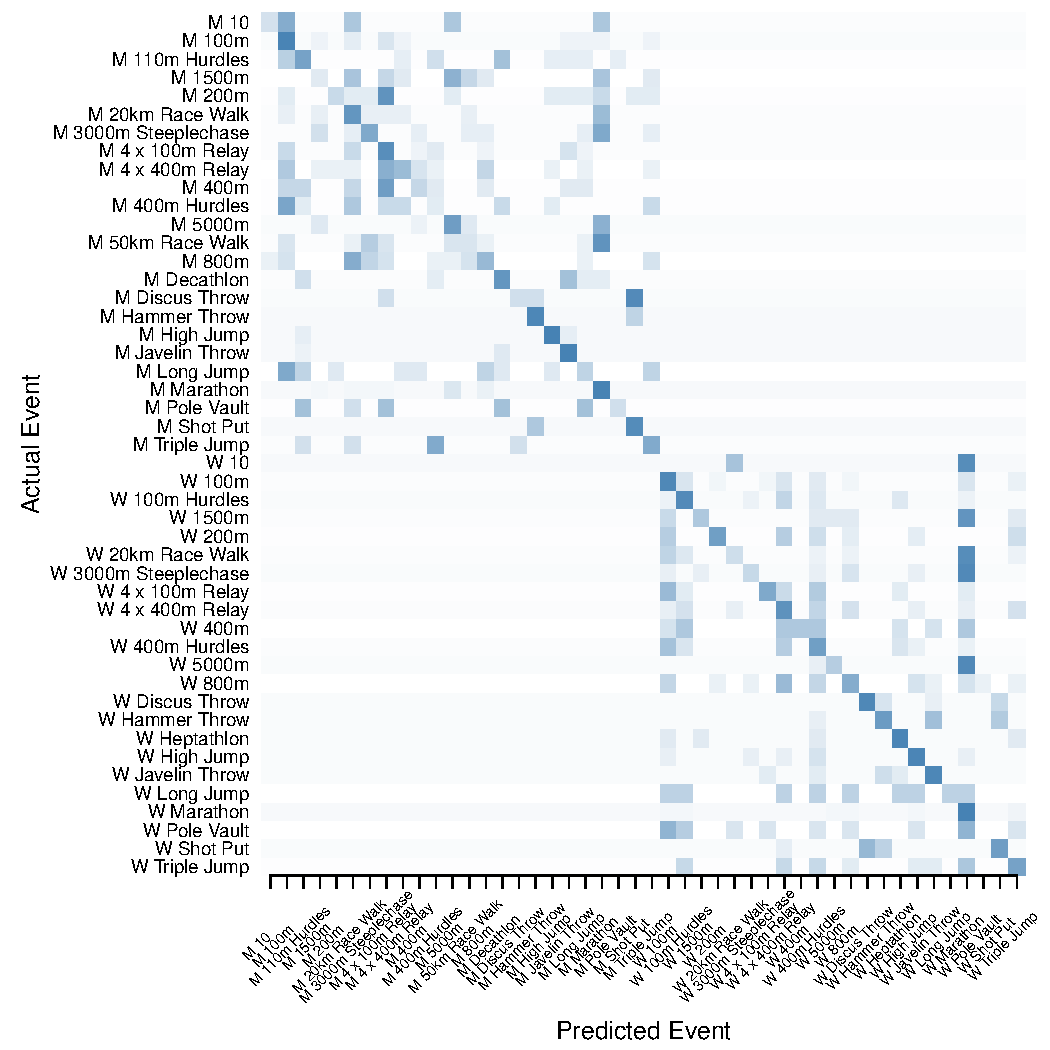
\includegraphics[scale=0.27]{../graphics/athletesANN-trn.pdf}
    \end{center}
  \end{minipage}
  \hspace{0.05\textwidth}
  \begin{minipage}{0.45\textwidth}
    \begin{center}
      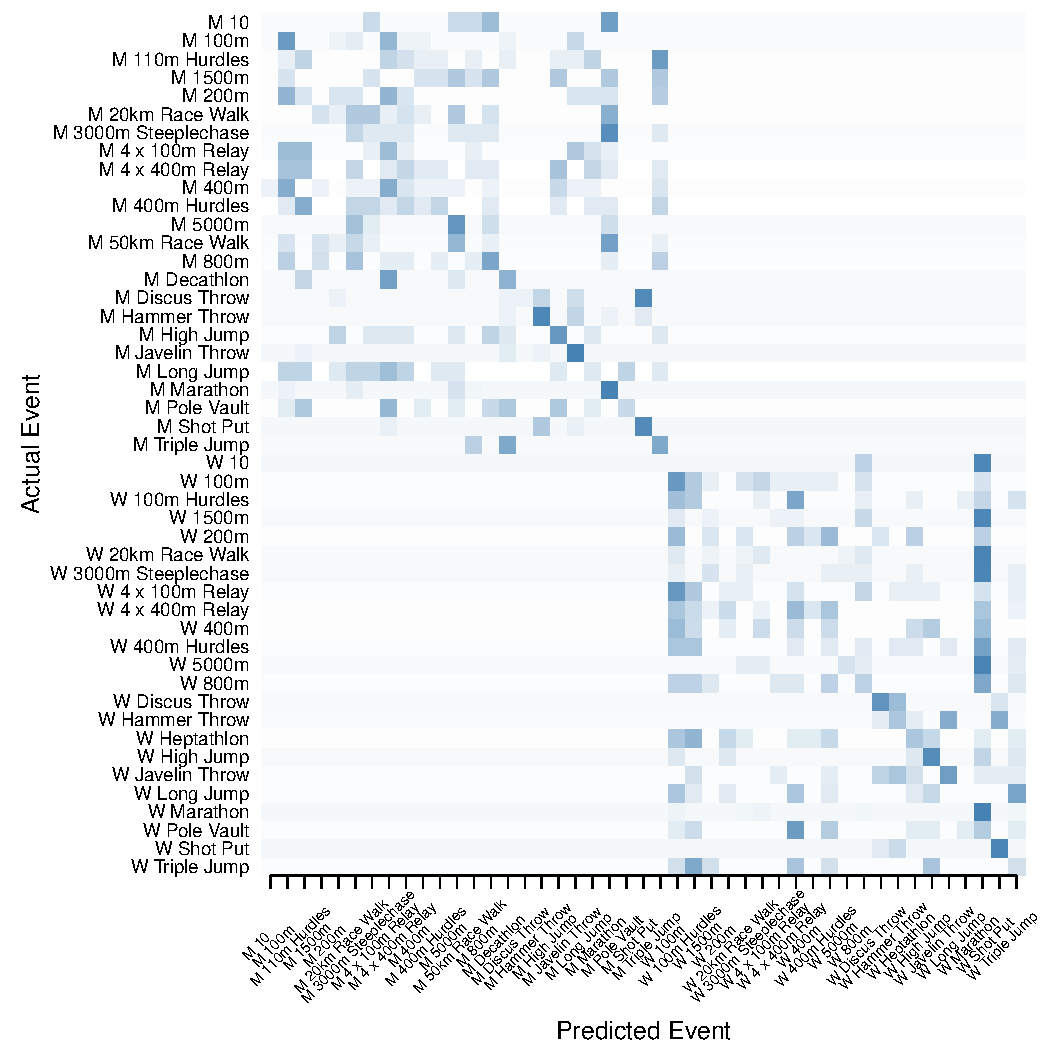
\includegraphics[scale=0.27]{../graphics/athletesANN-tst.pdf}
    \end{center}
  \end{minipage}
  \end{center}

 }

%%%%%%
  \headerbox{\bf Discussion}{name=conclusion,below=predictions,above=bottom,column=2}{
%%%%%
   \begin{itemize} \compresslist
      \item Classifying athletes by sport can be achieved with moderate accuracy using only a few features
      \item Additional features such as arm length and torso length could improve predictive accuracy
      % \item Data with a large number of categories can be difficult to classify
      \item Traits of athletes in some sports and events exhibit noticeable clustering, while other categories are less distinct (multi-modal)
      \item Above a minimum threshold of physicality, success in many sports is dependent on training
      \item Athletes in some sports and events have a well-defined body type, but Olympians exhibit a wide range of physical features
  \end{itemize}
 }

\end{poster}
\end{document}